\documentclass[a4paper,12pt]{article}
\usepackage[russian]{babel}

% Самые необходимые пакеты
\usepackage[T2A]{fontenc}
\usepackage[utf8]{inputenc}
\usepackage[russian]{babel}
\usepackage{geometry}
\usepackage{amsmath}
\usepackage{graphicx}
\usepackage{float} 
\usepackage{xcolor}
\usepackage{listings}
\usepackage{hyperref}
\usepackage{array}
\usepackage{caption}
\usepackage{booktabs}
\usepackage{amssymb}
\usepackage{subcaption}
\usepackage{caption}
\captionsetup[figure]{name=Рисунок}
\captionsetup[table]{name=Таблица}
\usepackage{pgfplots}
\pgfplotsset{compat=1.18}
\usetikzlibrary{arrows.meta}
\usepackage{capt-of}
\usepackage{multirow}
\usepackage[siunitx]{circuitikz}


\lstset{
	language=Matlab,
	basicstyle=\ttfamily\small,
	keywordstyle=\color{blue}\bfseries,
	commentstyle=\color{gray}\itshape,
	stringstyle=\color{red},
	numberstyle=\tiny\color{gray},
	numbers=left,
	stepnumber=1,
	numbersep=8pt,
	backgroundcolor=\color{white},
	frame=single,
	breaklines=true,
	breakatwhitespace=true,
	tabsize=4,
	showspaces=false,
	showstringspaces=false,
	captionpos=b,
	escapeinside={\%*}{*)},
}
\geometry{left=1.5cm, right=2cm, bottom=2cm, top=2cm}

\begin{document}
	
	% Титульный лист
	\begin{titlepage}
		\centering
		\vspace*{1cm}
		
		% Министерство
		{\small
			Министерство науки и высшего образования Российской Федерации\\
			Федеральное государственное автономное образовательное учреждение\\
			высшего образования\\
			«Национальный исследовательский университет ИТМО»\\
		}
		
		\vspace{2cm}
		
		% Факультет
		{\large
			Факультет систем управления и робототехники\\
		}
		
		\vspace{3cm}
		
		% Основной заголовок
		{\Huge\bfseries
			ОТЧЕТ\\
		}
		\vspace{0.5cm}
		{\LARGE\bfseries
			о лабораторной работе №5\\
		}
		
		\vspace{1cm}
		
		% Дисциплина и тема
		{\Large
			По дисциплине: «Линейные системы автоматического управления»\\
			\vspace{0.5cm}
			Тема: «Типовые динамические звенья»\\
		}
		
		\vspace{3cm}
		
		% Информация о студенте и преподавателях
		\begin{minipage}{0.4\textwidth}
			\raggedright
			{\large
				Студент:\\
			}
			Охрименко Е. Д.\\
			Поток: 1.1.3\\
			Вариант: 17\\
		\end{minipage}
		\hfill
		\begin{minipage}{0.4\textwidth}
			\raggedleft
			{\large
				Преподаватель:\\
			}
			Пашенко А. В.\\
		\end{minipage}
		
		\vfill
		
		% Город и год
		{\large
			Санкт-Петербург\\
			2025\\
		}
		
	\end{titlepage}
	
	\newpage
	\tableofcontents

	\newpage
	\section{Двигатель постоянного тока}
	
	
	
	Запишу уравнения для двигателя постоянного тока:
	\[
	J\dot{\omega} = M \qquad
	M = k_m I \qquad
	I = \frac{U + \varepsilon_i}{R} \qquad
	\varepsilon_i = -k_e \omega
	\]
	
	Тогда уравнение движения принимает вид:
	\[
	J\dot{\omega} = k_m I = k_m\frac{U - k_e \omega}{R}
	\]
	
	\[
	J\dot{\omega} + \frac{k_m k_e}{R}\,\omega = \frac{k_m}{R}U
	\]
	
	Выражу передаточную функцию:
	\[
	W(s)=
	\frac{\dfrac{k_m}{R}}{Js + \dfrac{k_m k_e}{R}}
	\]
	
	Теперь приведу её к стандартному виду
	\[
	W(s)=\frac{K}{Ts + 1}
	\]
	
	Для этого разделю числитель и знаменатель на \(\dfrac{k_m k_e}{R}\):
	\[
	W(s)=
	\frac{\dfrac{k_m}{R}}{\dfrac{k_m k_e}{R}}
	\cdot
	\frac{1}{\dfrac{J}{\dfrac{k_m k_e}{R}}s + 1}
	\]
	
	Отсюда параметры:
	\[
	K =
	\frac{\dfrac{k_m}{R}}{\dfrac{k_m k_e}{R}}
	= \frac{1}{k_e}
	\quad 
	T =
	\frac{J}{\dfrac{k_m k_e}{R}}
	= \frac{JR}{k_m k_e}
	\]
	
	Исходные значения, соответствующие моему варианту:
	\[
	k_m = 0.3074 \qquad
	k_e = 0.3074 \qquad
	J = 0.0019 \qquad
	R = 4.6730
	\]
	
	Вычислю постоянную времени:
	\[
	T = \frac{JR}{k_m k_e}
	= \frac{0.0019 \cdot 4.6730}{0.3074^2}
	\approx 0.094
	\]
	
	Коэффициент передачи:
	\[
	K = \frac{1}{k_e} = \frac{1}{0.3074} \approx 3.254
	\]
	
	Окончательная передаточная функция двигателя постоянного тока:
	\[
	W(s) = \frac{3.254}{0.094s + 1}
	\]
	
	Данная передаточная функция соответствует \textbf{апериодическому} звену первого порядка.
	
	\subsection{Временные характеристики}
	
	Весовая функция для апериодического звена первого порядка известна:
	
	\[
	w(t) = \frac{K}{T} e^{-t/T} = 34.63\, e^{-t/0.094}
	\]
	
	\begin{figure}[H]
		\centering
		
\includegraphics[width=0.9\textwidth]{../images/task1/time/w1.png}
		\caption{Весовая функция}
	\end{figure}
	
	И переходная функция: 
	\[
	h(t)=K \cdot \left(1-e^{-t/T}\right) = 3.254 \cdot \left(1-e^{-t/0.094}\right)	\]
	
	\begin{figure}[H]
		\centering
		
\includegraphics[width=0.9\textwidth]{../images/task1/time/y1.png}
		\caption{Переходная функция}
	\end{figure}
	
	\subsection{Частотные характеристики}
	
	Для получения частотных характеристик подставлю \(s = j\omega\):
	\[
	W(j\omega) = \frac{K}{1 + j\omega T}
	\]
	
	Амплитудно-частотная характеристика определяется модулем комплексной функции:
	\[
	A(\omega) = |W(j\omega)|
	= \frac{K}{\sqrt{1 + (\omega T)^2}}
	\]
	
	Подставим численные значения параметров:
	\[
	A(\omega)
	= \frac{3.254}{\sqrt{1 + \omega^2 \cdot 0.094^2}}
	= \frac{3.254}{\sqrt{1 + 0.008836\,\omega^2}}
	\]
	
	\begin{figure}[H]
		\centering
		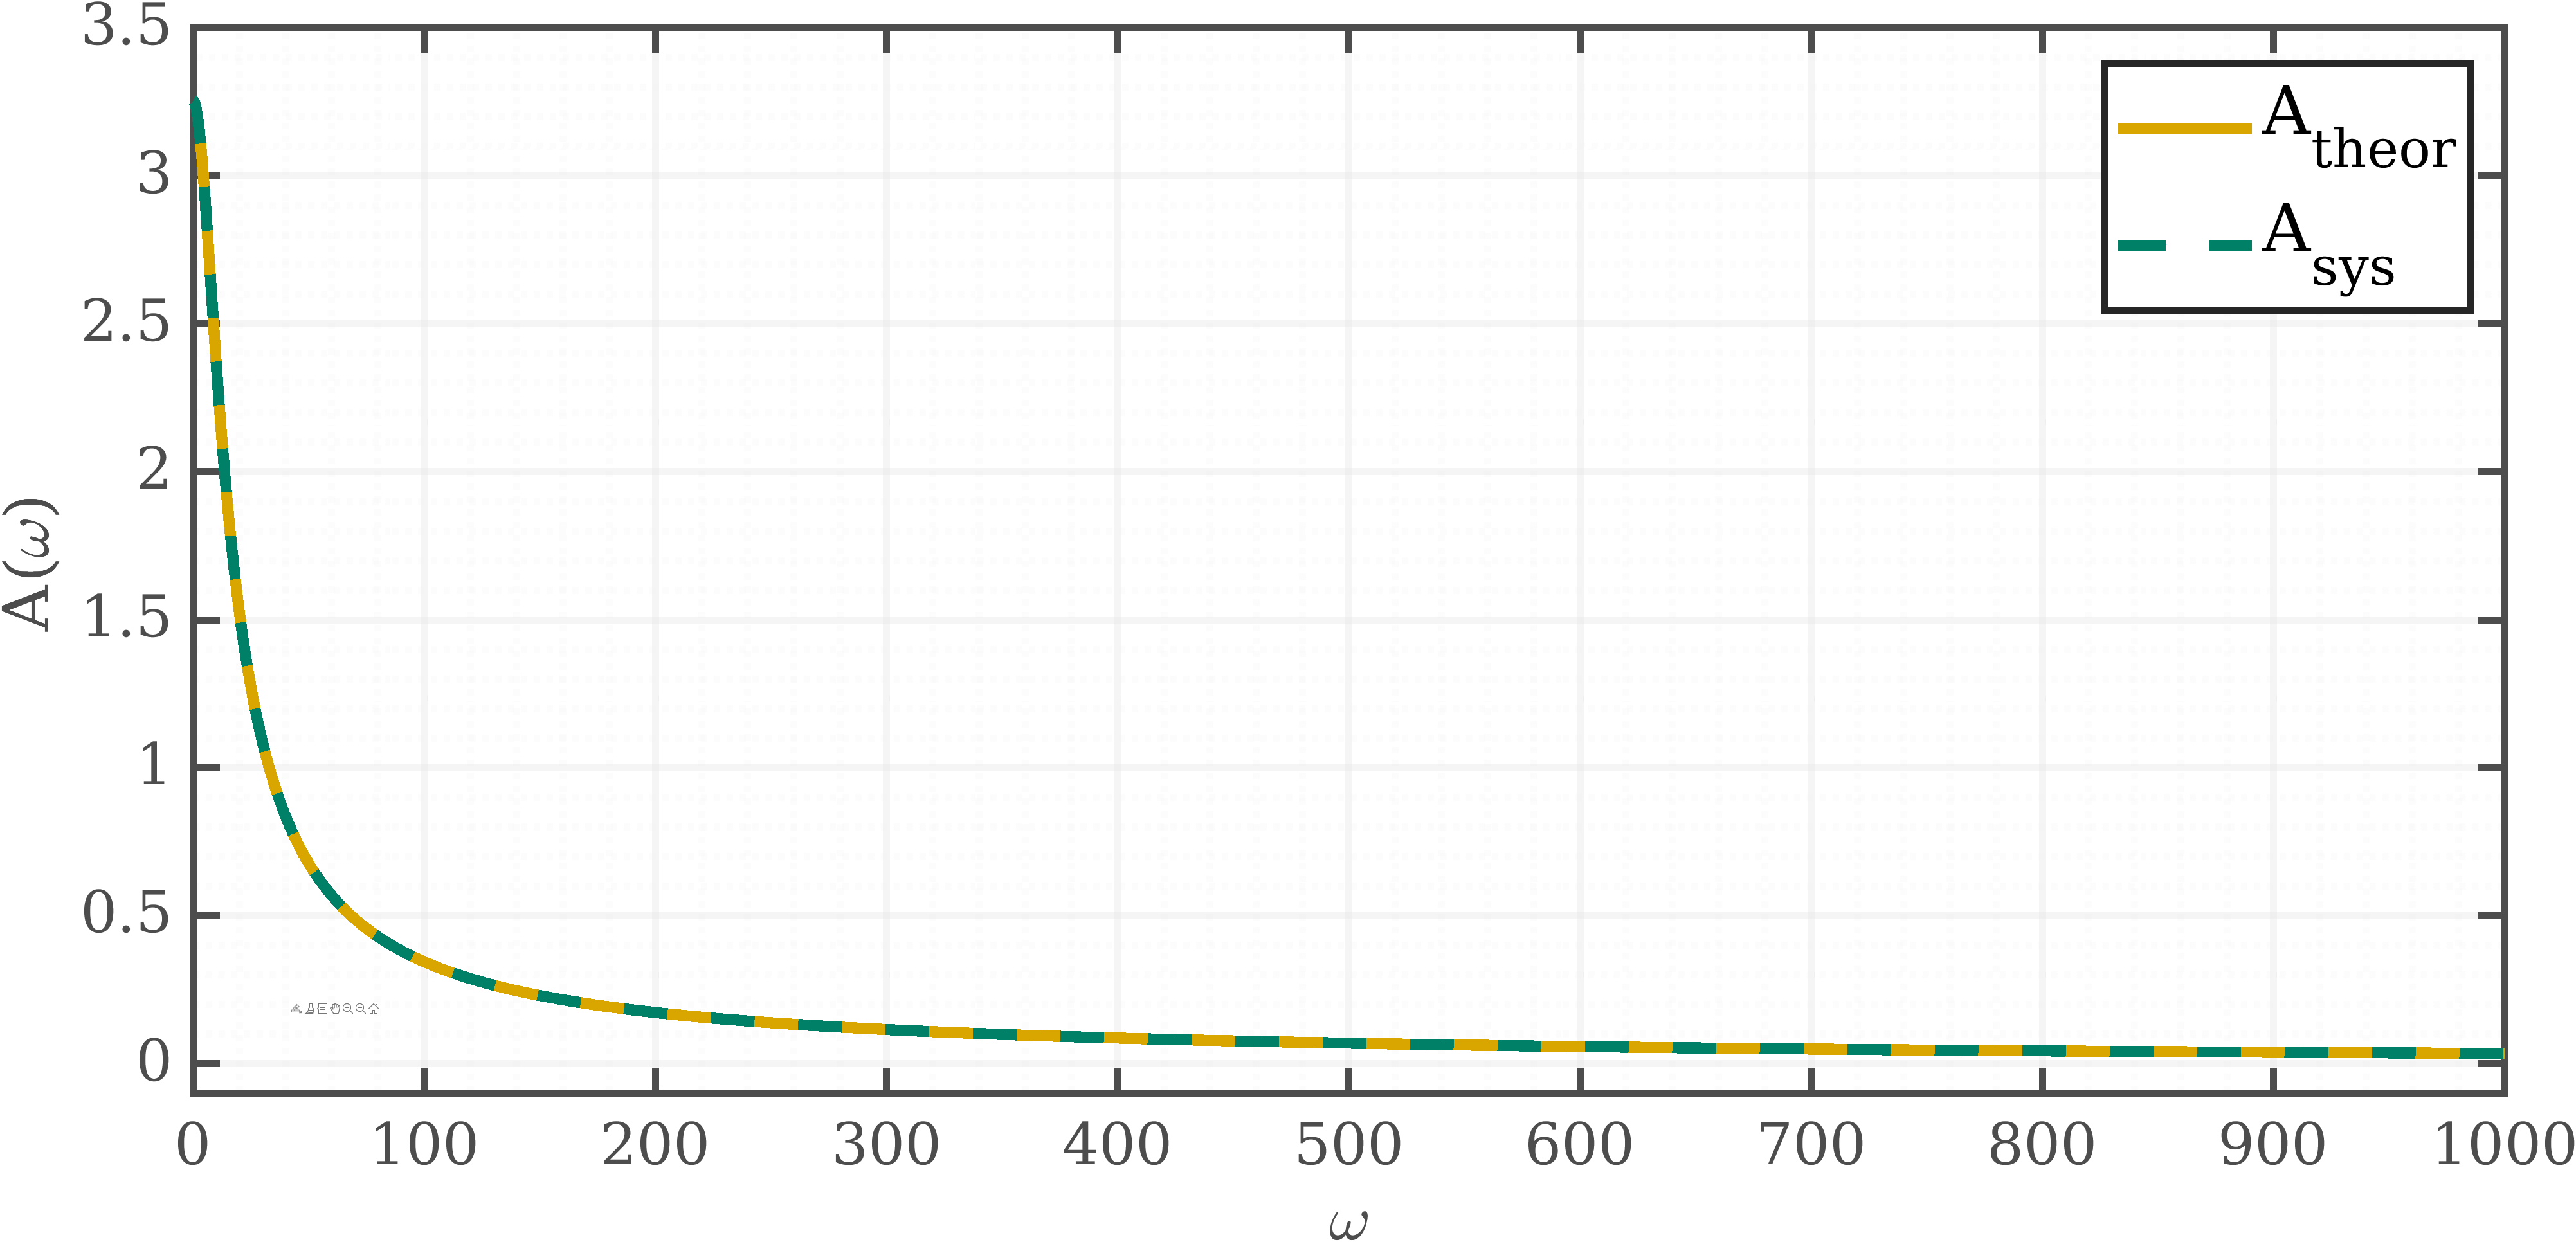
\includegraphics[width=0.9\textwidth]{../images/task1/freq/ach1.png}
		\caption{АЧХ}
	\end{figure}
	
	Логарифмическая амплитудно-частотная характеристика (ЛАЧХ)
	определяется выражением
	\[
	L(\omega)=20\lg A(\omega)
	\qquad 
	A(\omega)=\frac{K}{\sqrt{1+(\omega T)^2}}
	\]
	
	ЛАЧХ имеет вид:
	
	\[
	L(\omega)=
	20\lg
	\left(
	\frac{3.254}{\sqrt{1 + 0.008836\,\omega^2}}
	\right)
	\]
	
	\begin{figure}[H]
		\centering
		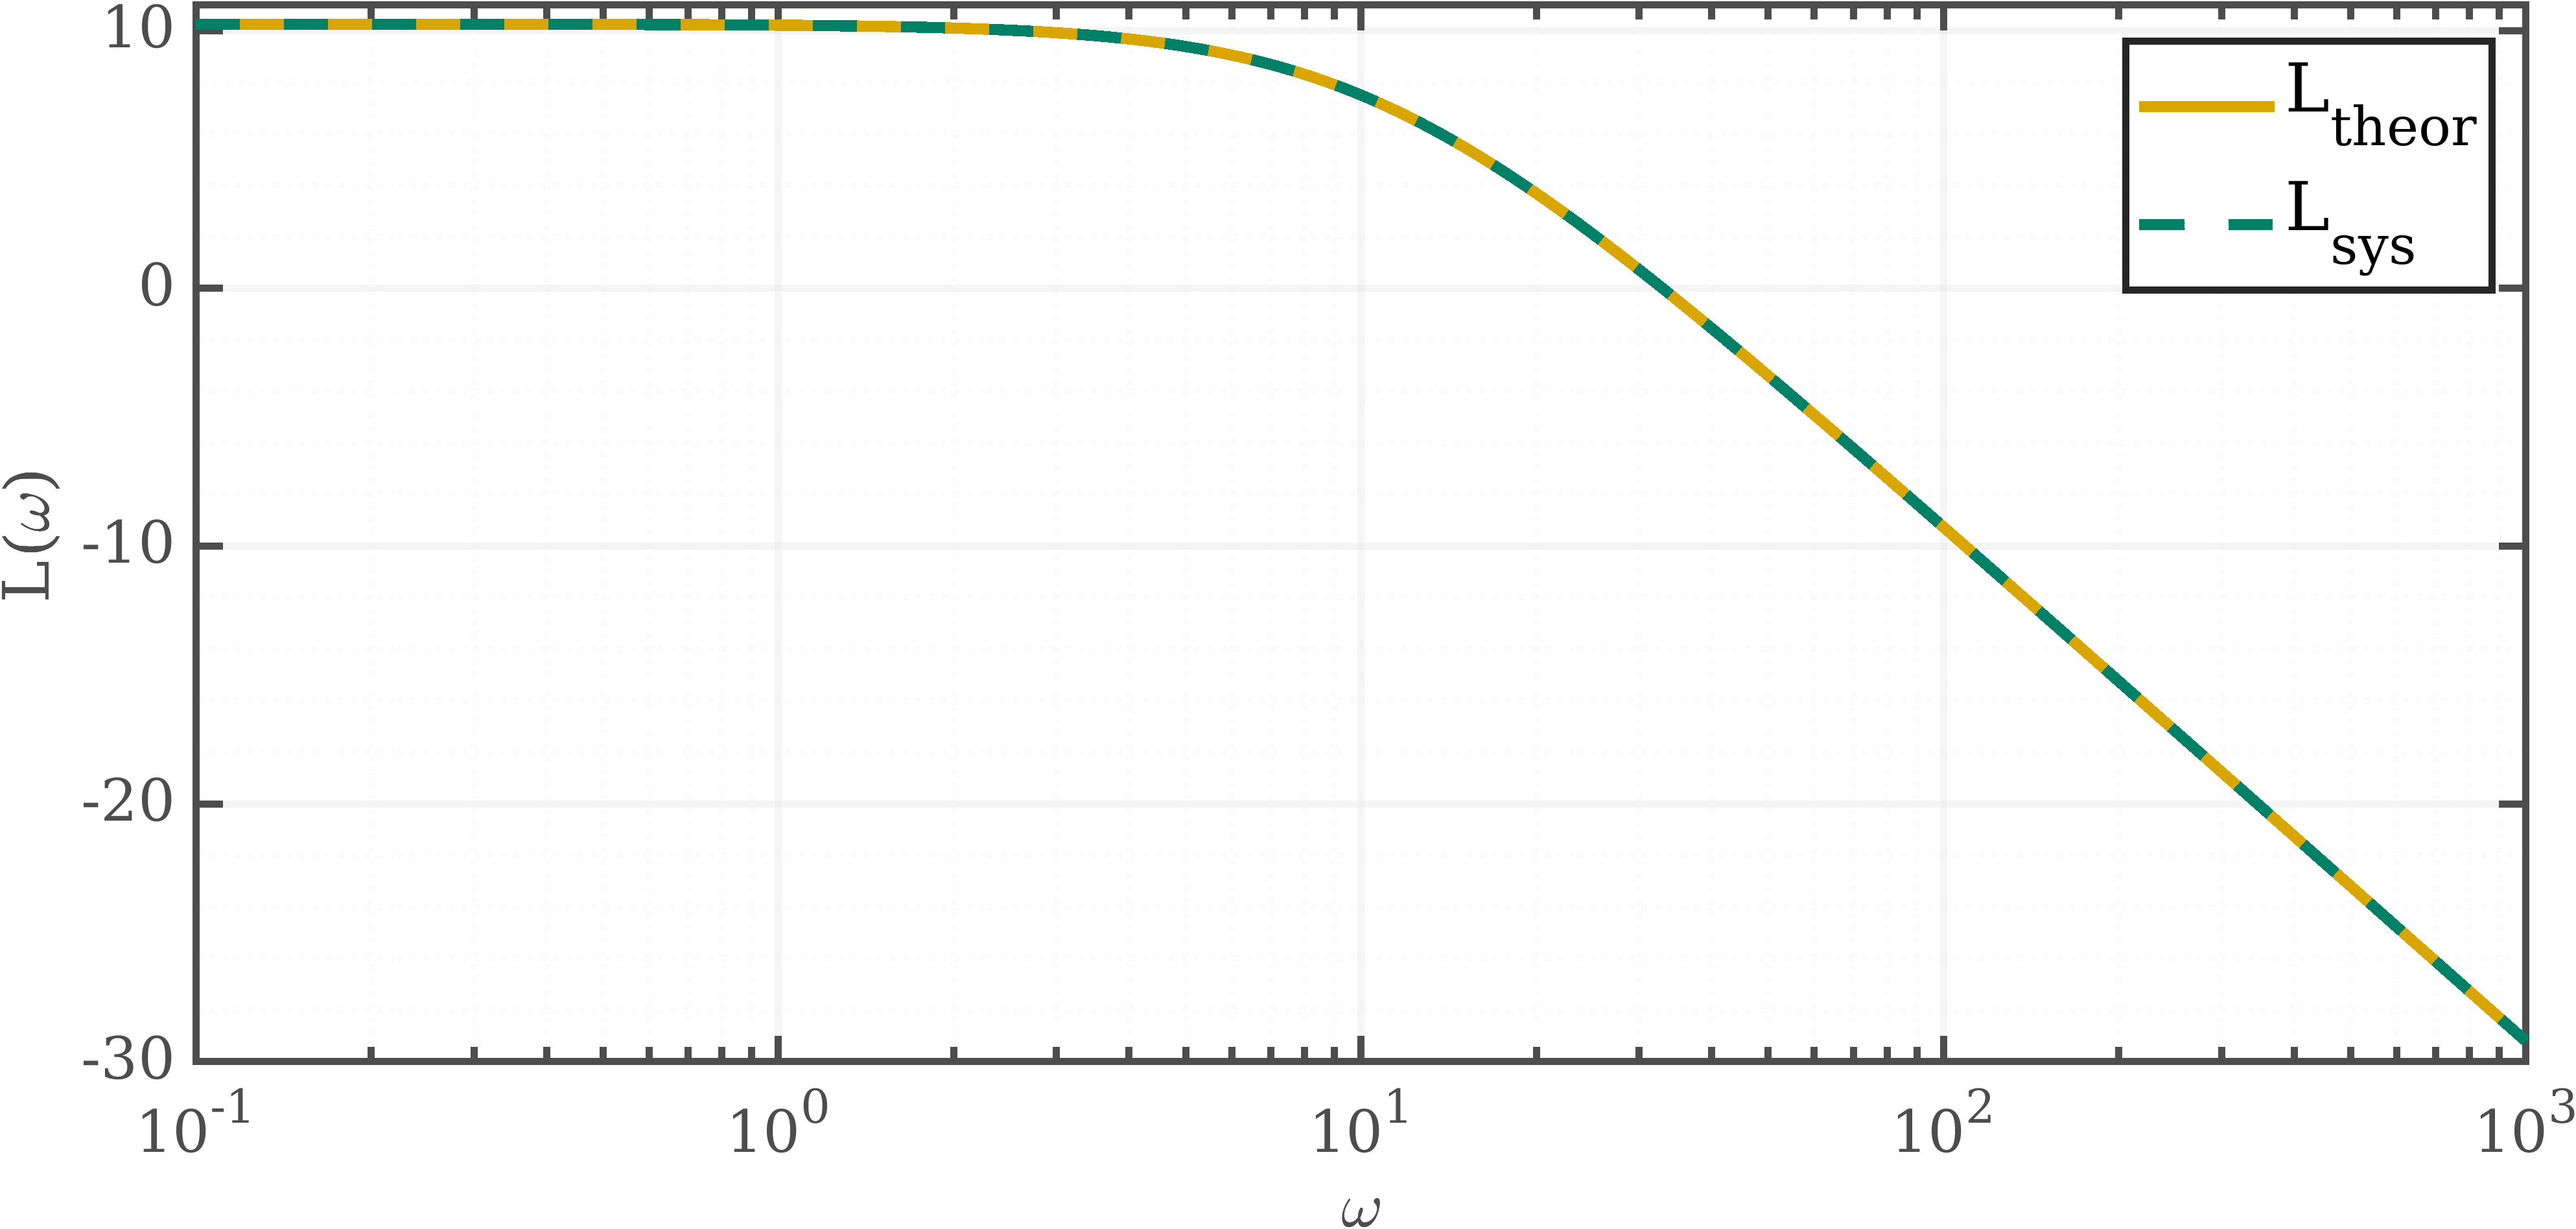
\includegraphics[width=0.9\textwidth]{../images/task1/freq/lach1.png}
		\caption{ЛАЧХ}
	\end{figure}

	
	
	Фазо-частотная характеристика (ФЧХ) определяется аргументом комплексной частотной функции. Для апериодического звена первого порядка:
	
	\[
	\varphi(\omega) = -\,\arctan(\omega T)
	\]
	
	Подставлю численное значение постоянной времени:
	\[
	\varphi(\omega) = -\arctan(0.094\,\omega)
	\]
	
	\begin{figure}[H]
		\centering
		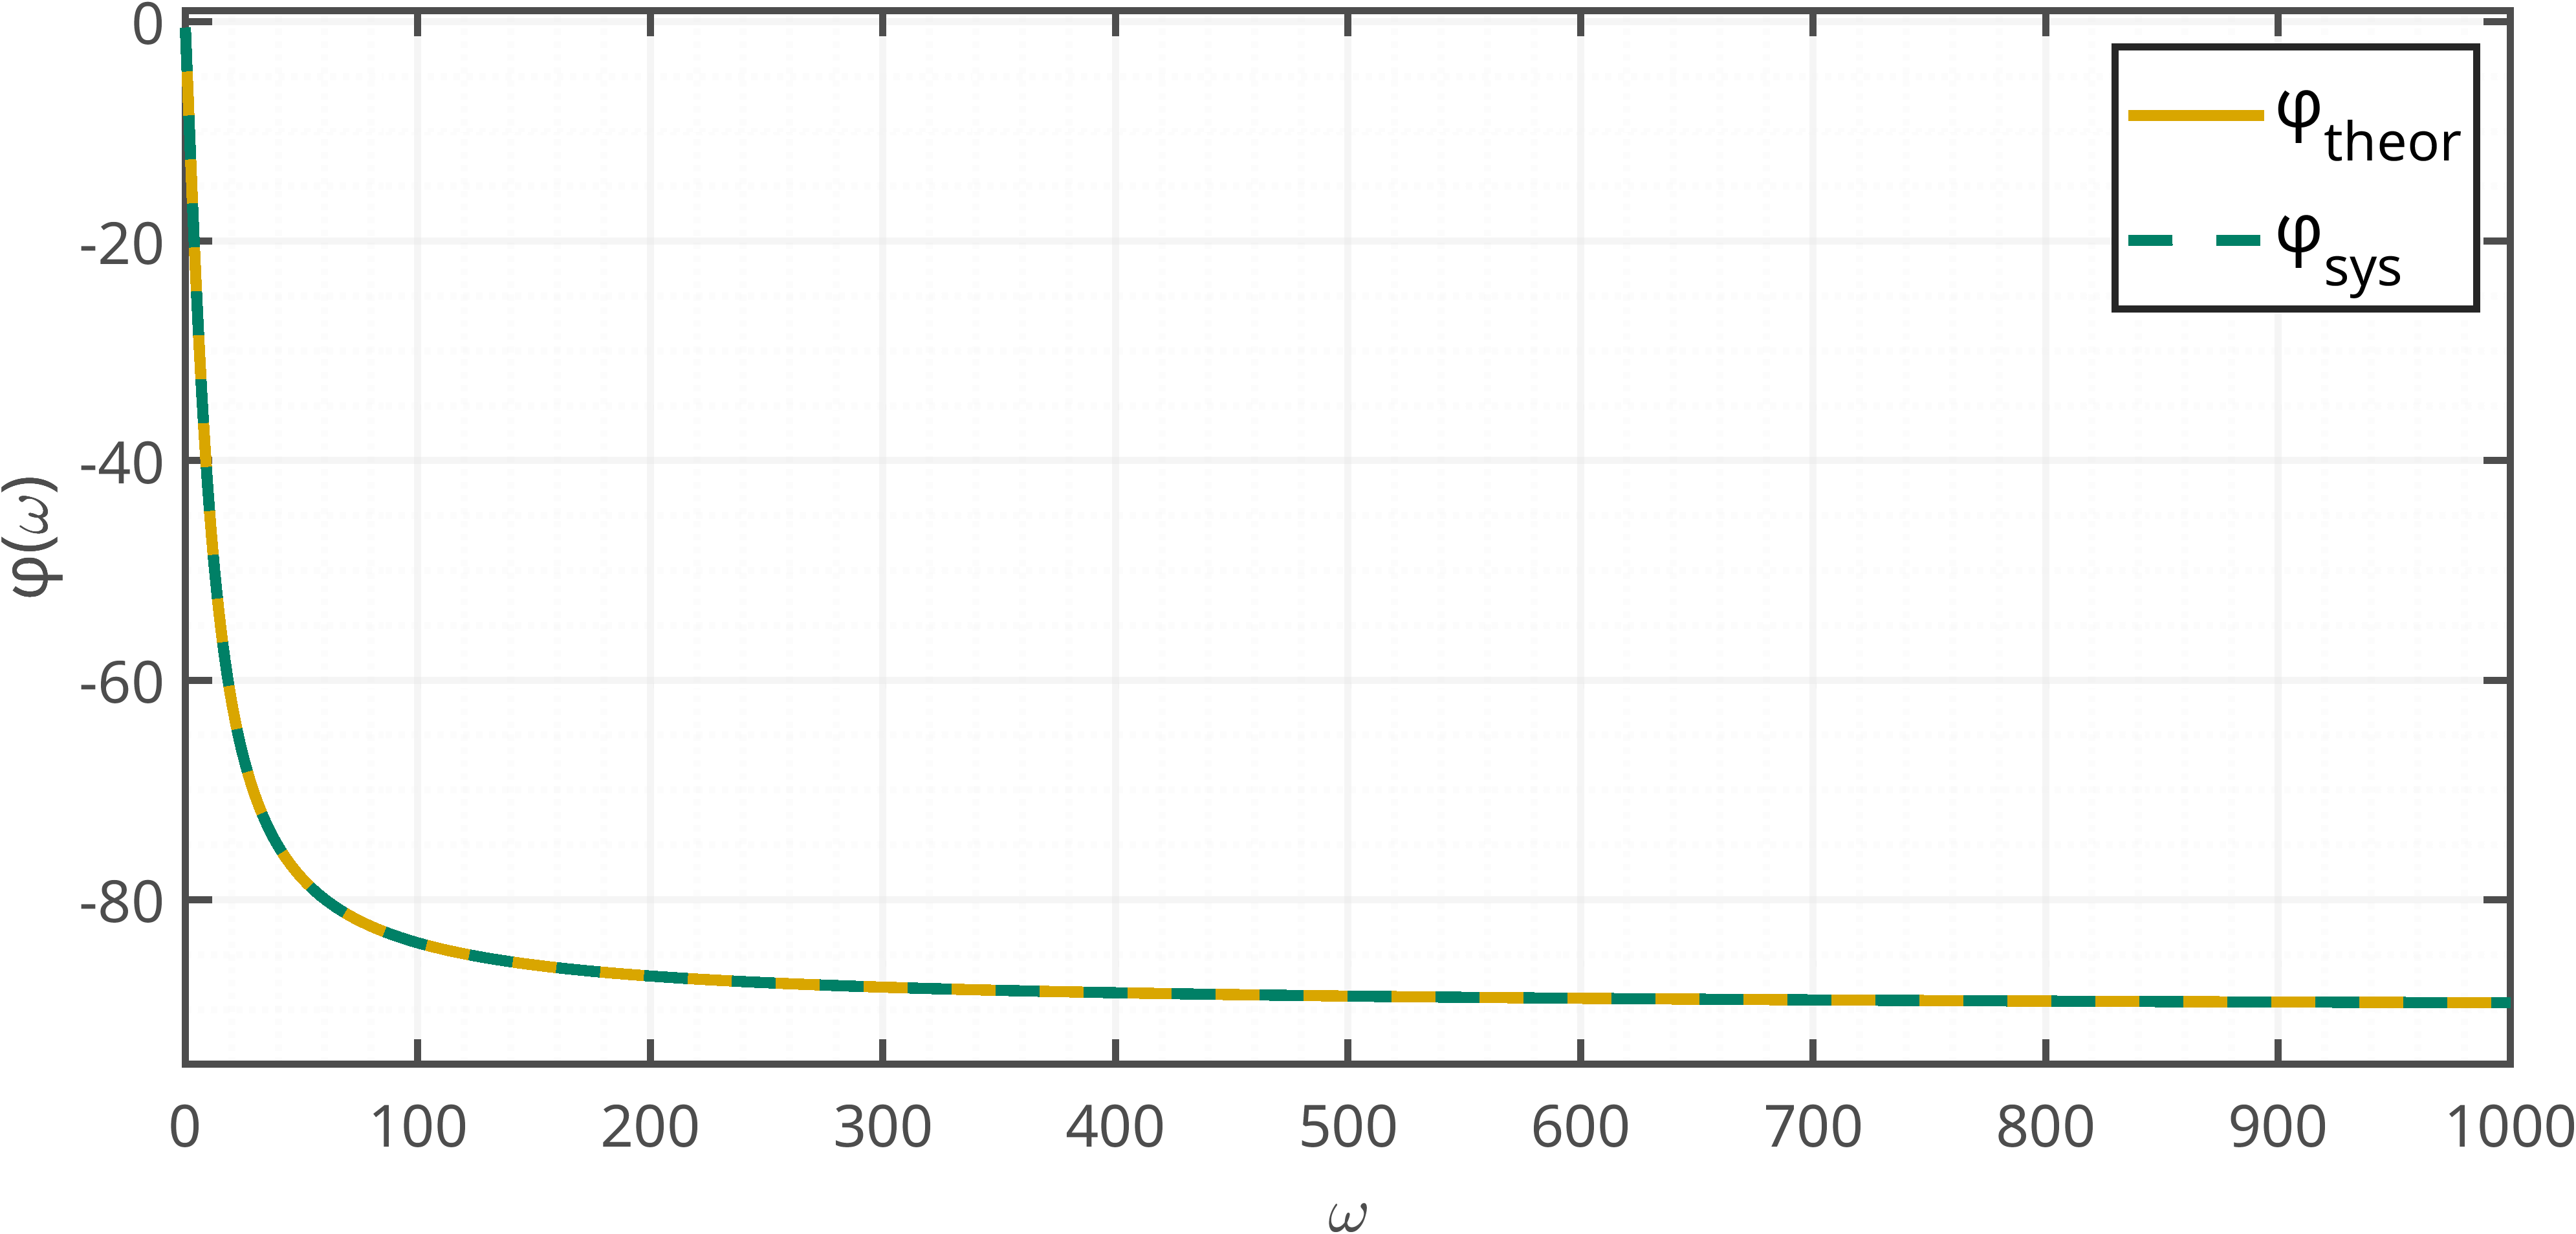
\includegraphics[width=0.9\textwidth]{../images/task1/freq/fch1.png}
		\caption{ФЧХ}
	\end{figure}
	
	Логарифмическая фазо-частотная характеристика (ЛФЧХ) строится как зависимость 
	фазовой характеристики \(\varphi(\omega)\) от логарифма частоты \(\omega\).
	
	ЛФЧХ имеет тот же аналитический вид
	\[
	\varphi(\omega) = -\arctan(0.094\,\omega)
	\]
	но строится в координатах
	\[
	\left( \lg\omega,\;\varphi(\omega) \right)
	\]
	
	\begin{figure}[H]
		\centering
		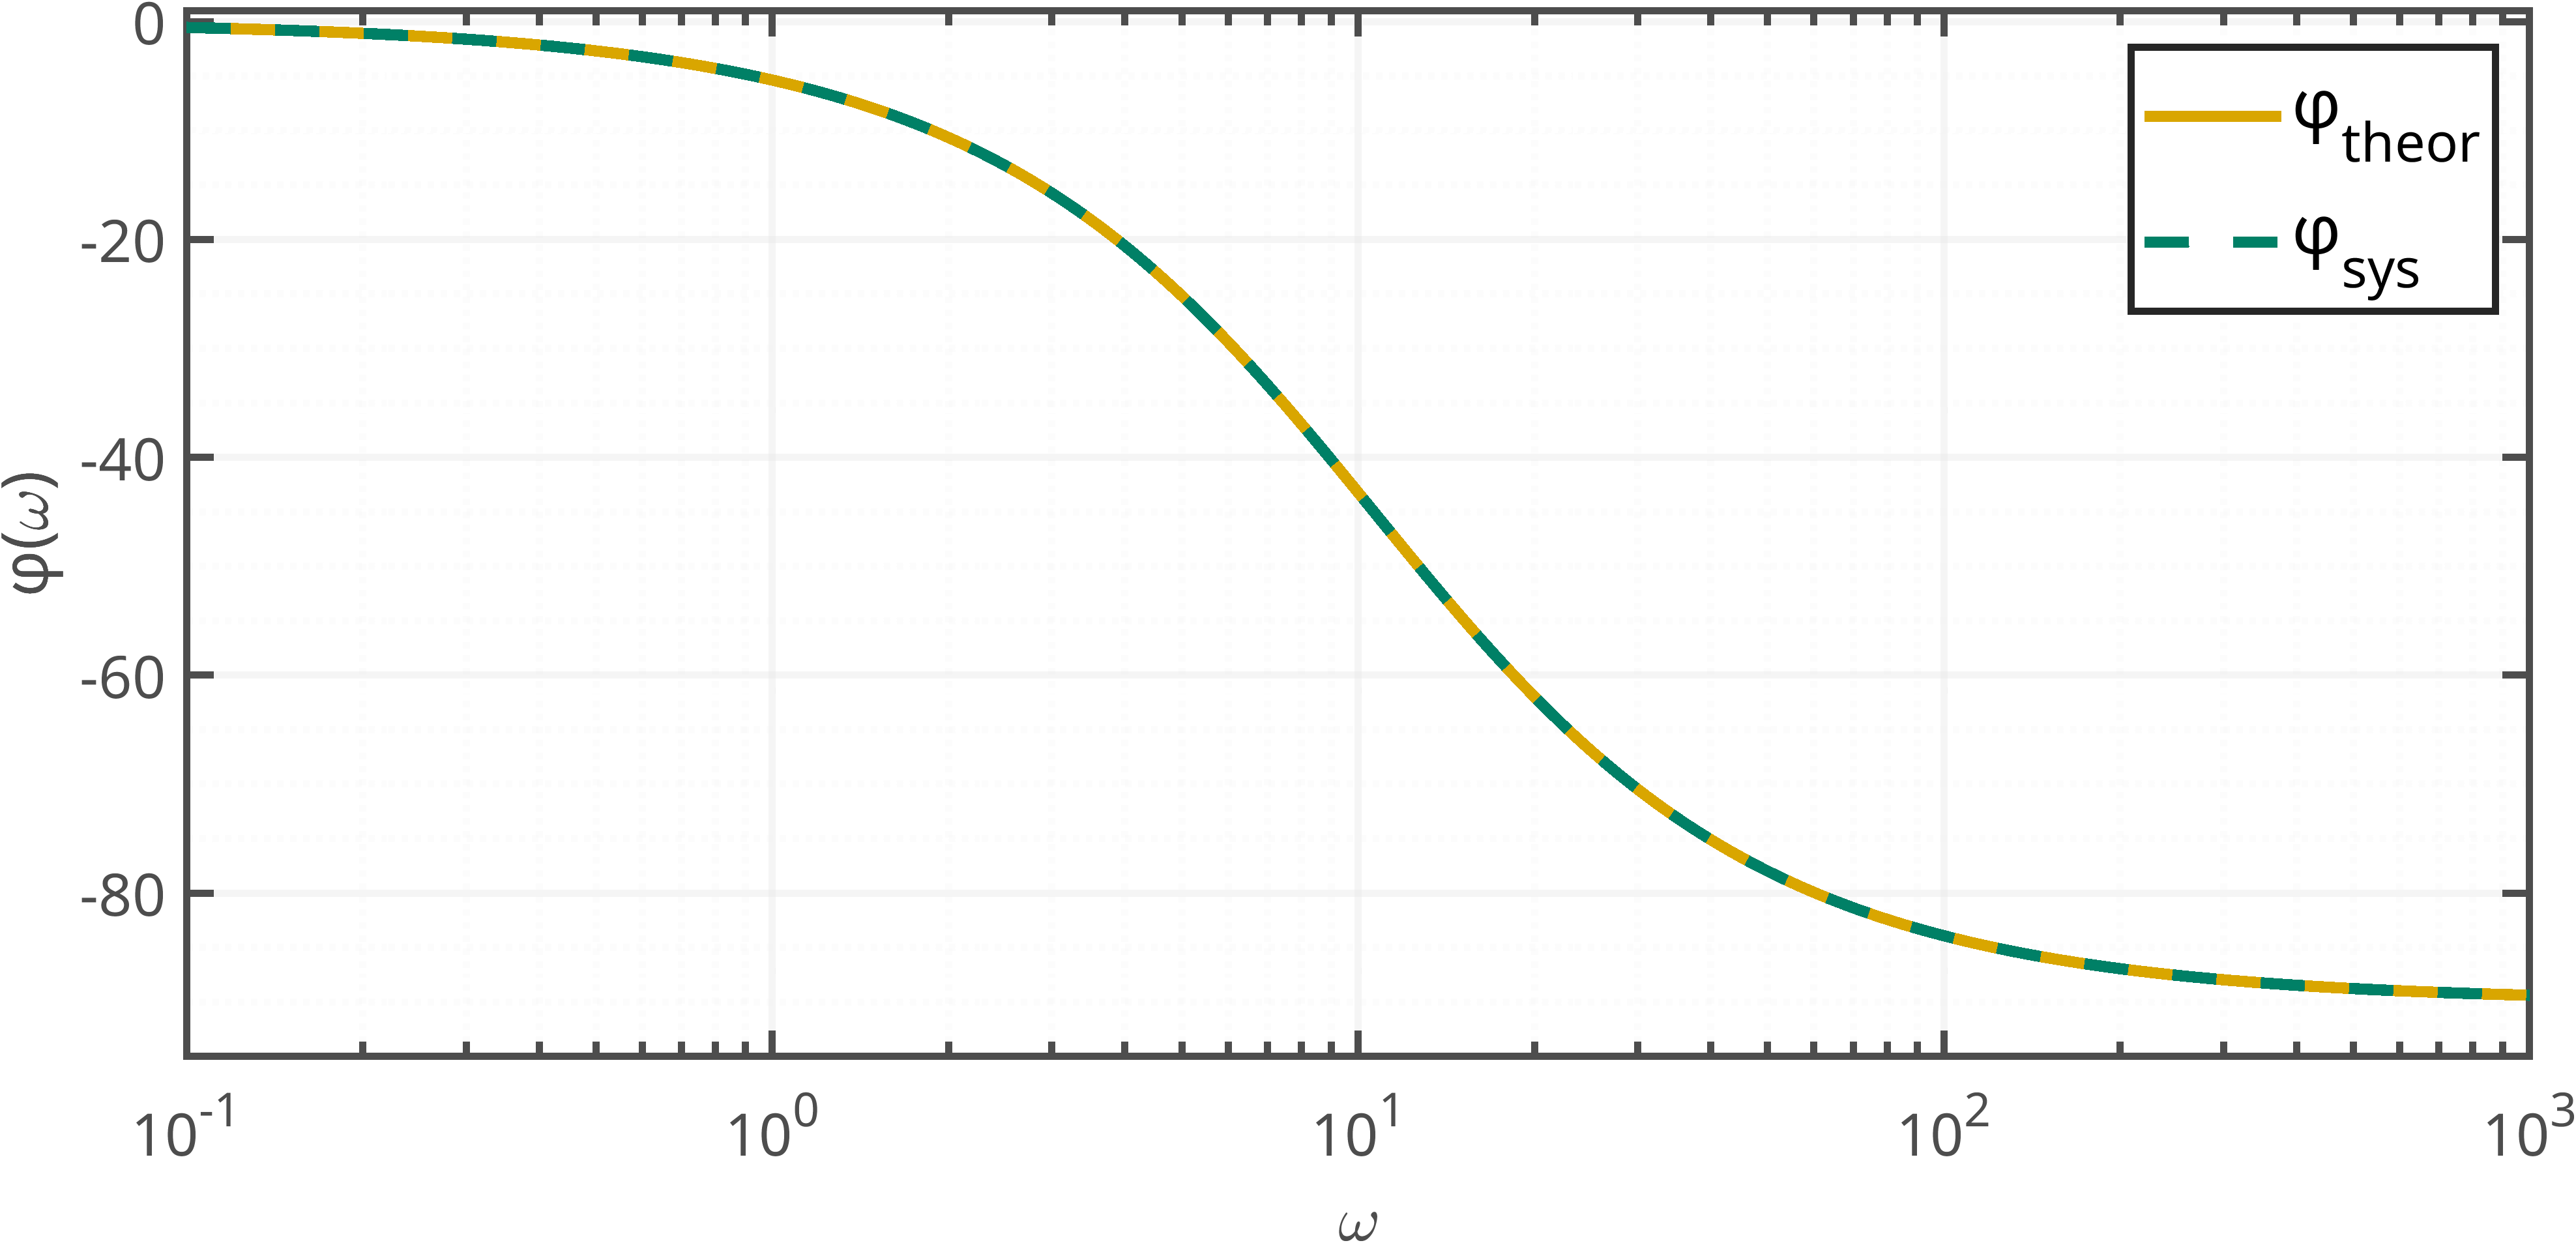
\includegraphics[width=0.9\textwidth]{../images/task1/freq/lfch1.png}
		\caption{ЛФЧХ}
	\end{figure}
	
	\textbf{Итог: } 
	
	\newpage
	\section{Двигатель постоянного тока 2.0}
	
	Запишу уравнения двигателя постоянного тока независимого возбуждения:
	\[
	J\dot{\omega} = M \qquad
	M = k_m I \qquad
	I = \frac{U + \varepsilon}{R}
	\]
	\[
	\varepsilon = \varepsilon_i + \varepsilon_s \qquad
	\varepsilon_i = -k_e \omega \qquad
	\varepsilon_s = -L\dot{I}
	\]
	
	Дифференциальное уравнение объекта:
	\[
	\frac{JL}{k_m}\ddot{\omega}
	+ \frac{JR}{k_m}\dot{\omega}
	+ k_e\omega = U
	\]
	
	Передаточная функция:
	\[
	W(s) = 
	\frac{1}{
		\displaystyle
		\frac{JL}{k_m}s^2
		+ \frac{JR}{k_m}s
		+ k_e }
	\]
	
	Разделю числитель и знаменатель на \(k_e\),
	чтобы привести выражение к нормированному виду:
	\[
	W(s) =
	\frac{1}{k_e}\,
	\frac{1}{
		\displaystyle
		\frac{JL}{k_m k_e}s^2
		+ \frac{JR}{k_m k_e}s
		+ 1 }
	\]
	
	Теперь приведу ПФ двигателя к стандартной форме
	колебательного звена:
	
	\[
	W(s) = \frac{K}{T^2 s^2 + 2\xi T s + 1 }
	\]
	
	Сравнивая коэффициенты, получаю параметры:
	
	\[
	K = \frac{1}{k_e}
	\qquad
	T^2 = \frac{JL}{k_m k_e}
	\qquad
	2\xi T = \frac{JR}{k_m k_e}
	\]
	
	Отсюда:
	
	\[
	T = \sqrt{\frac{JL}{k_m k_e}}
	\qquad
	\xi = 
	\frac{JR}{2 k_m k_e T}
	=
	\frac{JR}{2 k_m k_e \sqrt{\dfrac{JL}{k_m k_e}}}
	\]
	
	Подставлю значения своего варианта:
	
	\[
	K = \frac{1}{k_e} \approx 3.25
	\qquad
	T = \sqrt{ \frac{JL}{k_m k_e} } \approx 0.144
	\qquad
	\xi = \frac{JR}{2k_m k_e T} \approx 0.33
	\]
	
	Передаточная функция:
	
	\[
	W(s) = 
	\frac{3.25}{0.0208 s^2 + 0.094 s + 1}
	\]\\
	
	Тип звена: \textbf{колебательное} (\(0 < \xi = 0.33 < 1\)).
	
	\subsection{Временные характеристики}
	
	Весовая функция колебательного звена равна:
	
	\[
	w(t) = \frac{K}{T\sqrt{1-\xi^{2}}}\,
	e^{-\dfrac{\xi t}{T}}\,
	\sin\!\left(\frac{\sqrt{1-\xi^{2}}}{T}\,t\right)\qquad t>0
	\]
	
	Для моего варианта:
	
	\[
	w(t) \approx 23.9\,e^{-2.29t}\,\sin(6.56t) \qquad t>0
	\]
	
	\begin{figure}[H]
		\centering
		
\includegraphics[width=0.9\textwidth]{../images/task2/time/w2.png}
		\caption{Весовая функция}
	\end{figure}
	
	Переходная функция колебательного звена:
	
	\[
	h(t)
	=
	K\!\left[
	1
	-
	e^{-\frac{\xi}{T} t}
	\left(
	\cos\!\left(\frac{\sqrt{1-\xi^{2}}}{T}\,t\right)
	+
	\frac{\xi}{\sqrt{1-\xi^{2}}}
	\sin\!\left(\frac{\sqrt{1-\xi^{2}}}{T}\,t\right)
	\right)
	\right] \qquad t>0
	\]
	
	Мои значения:
	
	\[
	h(t)
	=
	3.254\!\left[
	1
	-
	e^{-2.29 t}
	\left(
	\cos(6.56\,t)
	+
	0.3494\,\sin(6.56\,t)
	\right)
	\right] \qquad t>0
	\]
	
	\begin{figure}[H]
		\centering
		
\includegraphics[width=0.9\textwidth]{../images/task2/time/y2.png}
		\caption{Переходная функция}
	\end{figure}	

	\subsection{Частотные характеристики}
	
	Запишу АЧХ колебательного звена
	
	\[
	A(\omega) = \frac{K}{\sqrt{\bigl(1 - \omega^2 T^2\bigr)^2 + \bigl(2\xi \omega T\bigr)^2}}
	\]
	
	Подставлю мои значения:
	
	\[
	A(\omega) =
	\frac{3.25}{\sqrt{\bigl(1 - 0.0208\,\omega^2\bigr)^2 + \bigl(0.095\,\omega\bigr)^2}}
	\]
	
	\begin{figure}[H]
		\centering
		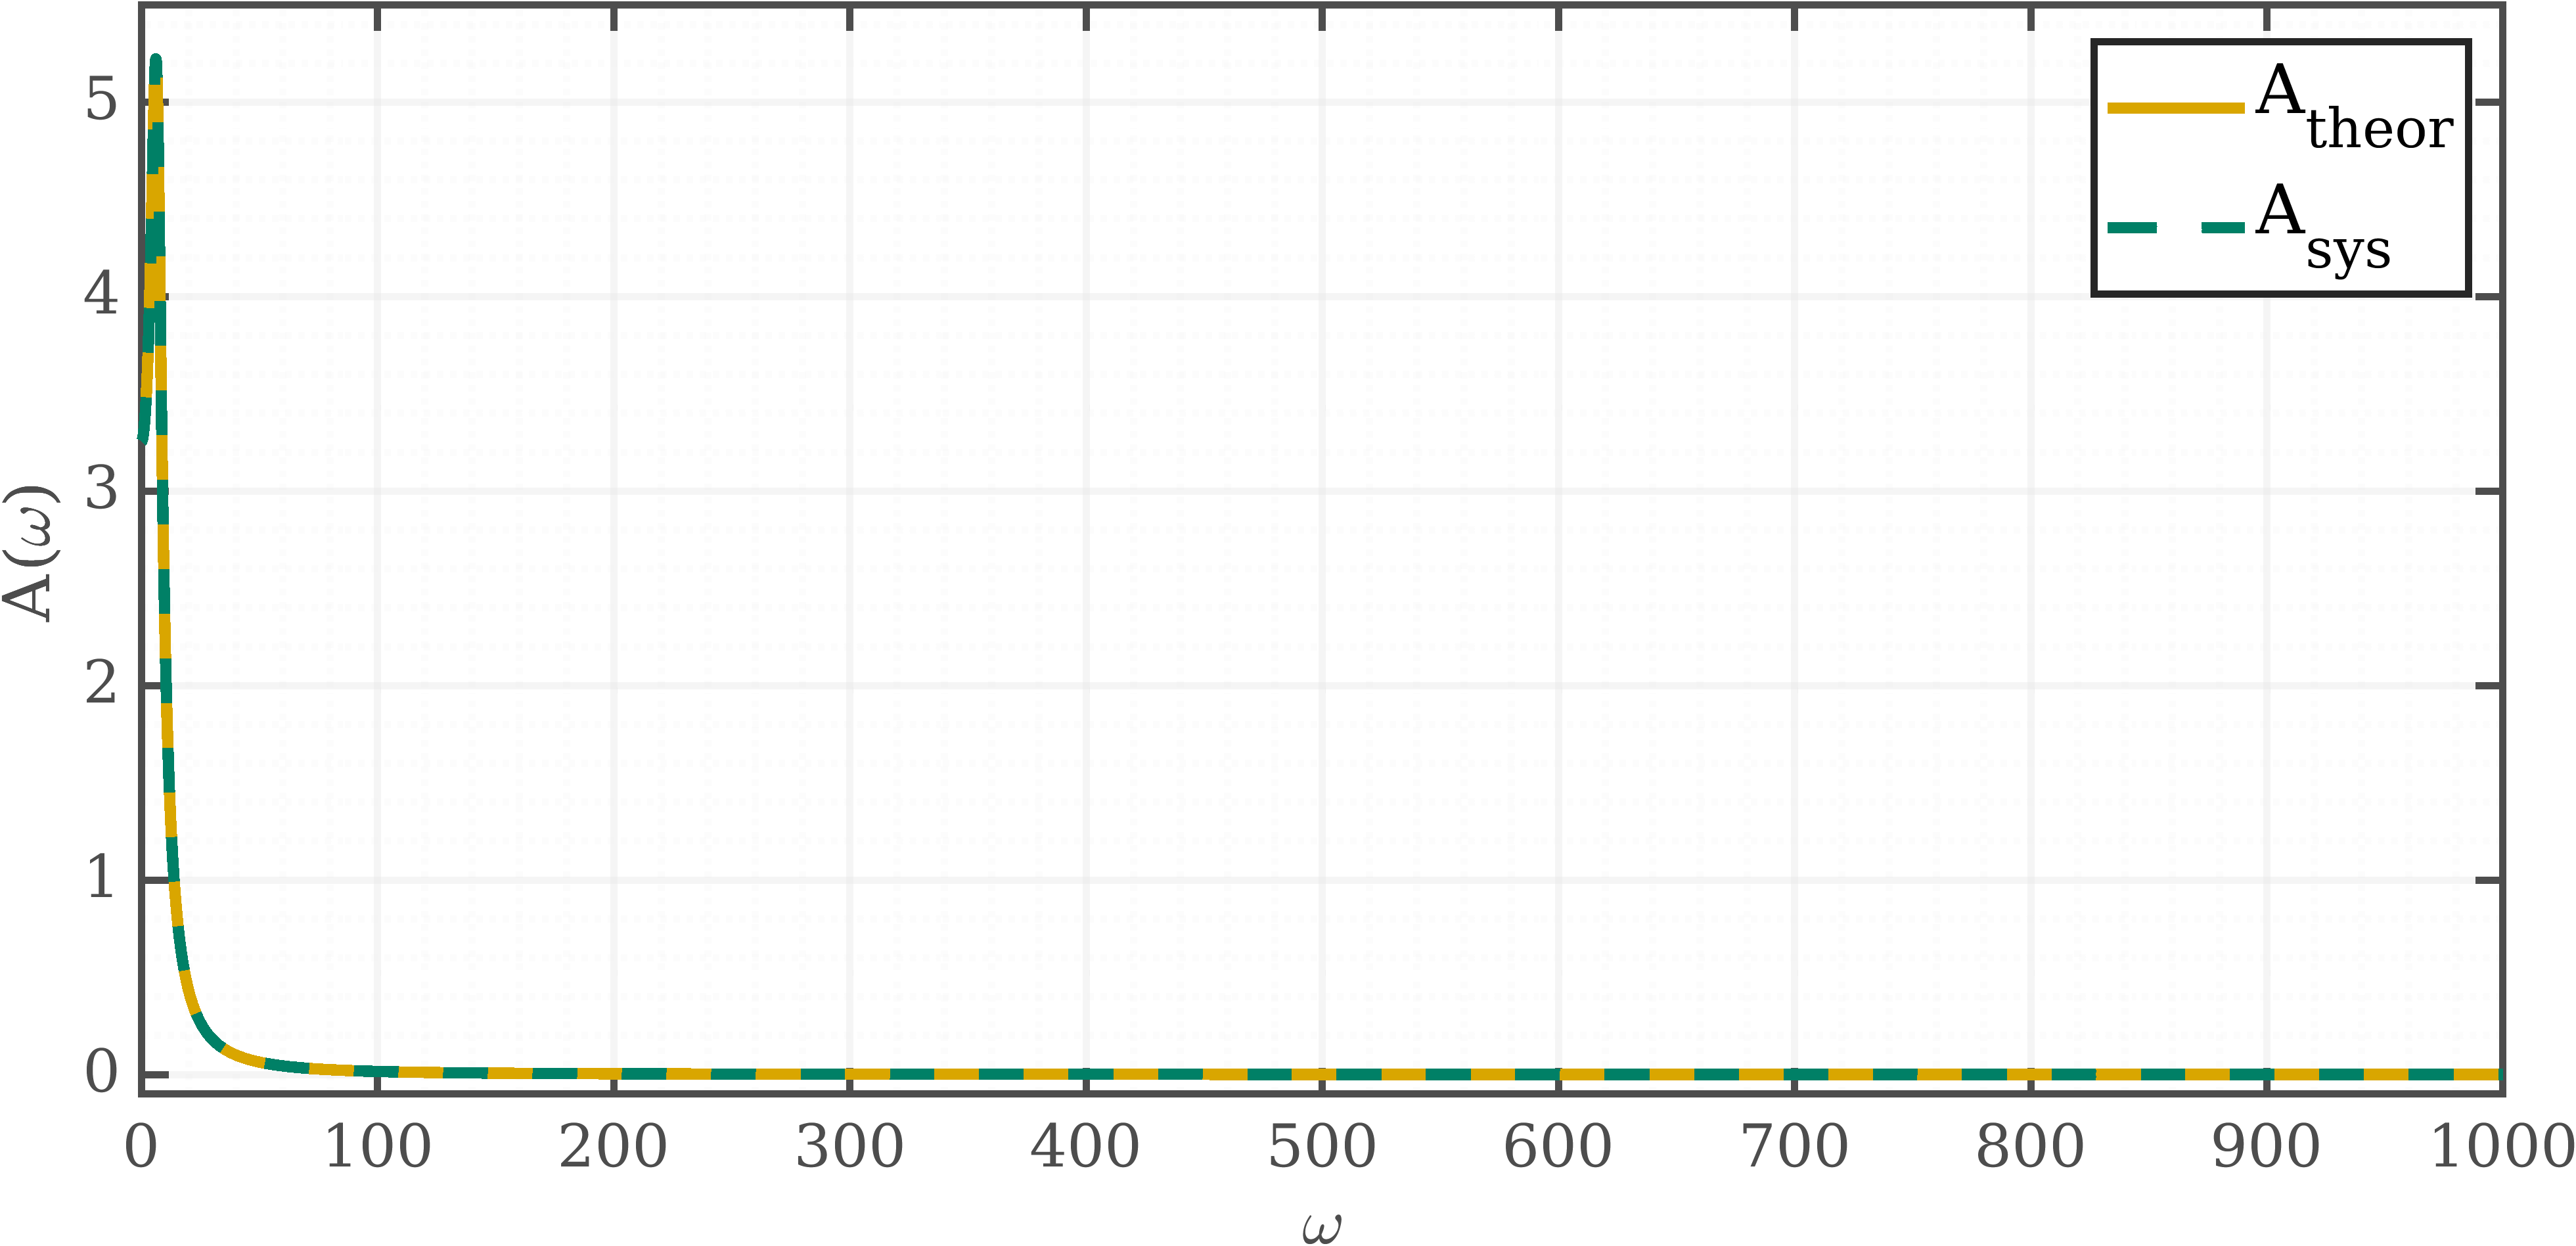
\includegraphics[width=0.9\textwidth]{../images/task2/freq/ach2.png}
		\caption{АЧХ}
	\end{figure}	
	
	ЛАЧХ колебательного звена:
	
	\[
	L(\omega)
	=
	20\lg K
	-
	10\lg\!\left[
	\left(1-\omega^{2}T^{2}\right)^{2}
	+
	4\xi^{2}\omega^{2}T^{2}
	\right]
	\]
	
	С моими значениями:
	
	\[
	L(\omega)
	=
	20\lg(3.254)
	-
	10\lg\!\left[
	\left(1 - 0.0207\,\omega^{2}\right)^{2}
	+
	0.00908\,\omega^{2}
	\right]
	\]
	
	
		
	\begin{figure}[H]
		\centering
		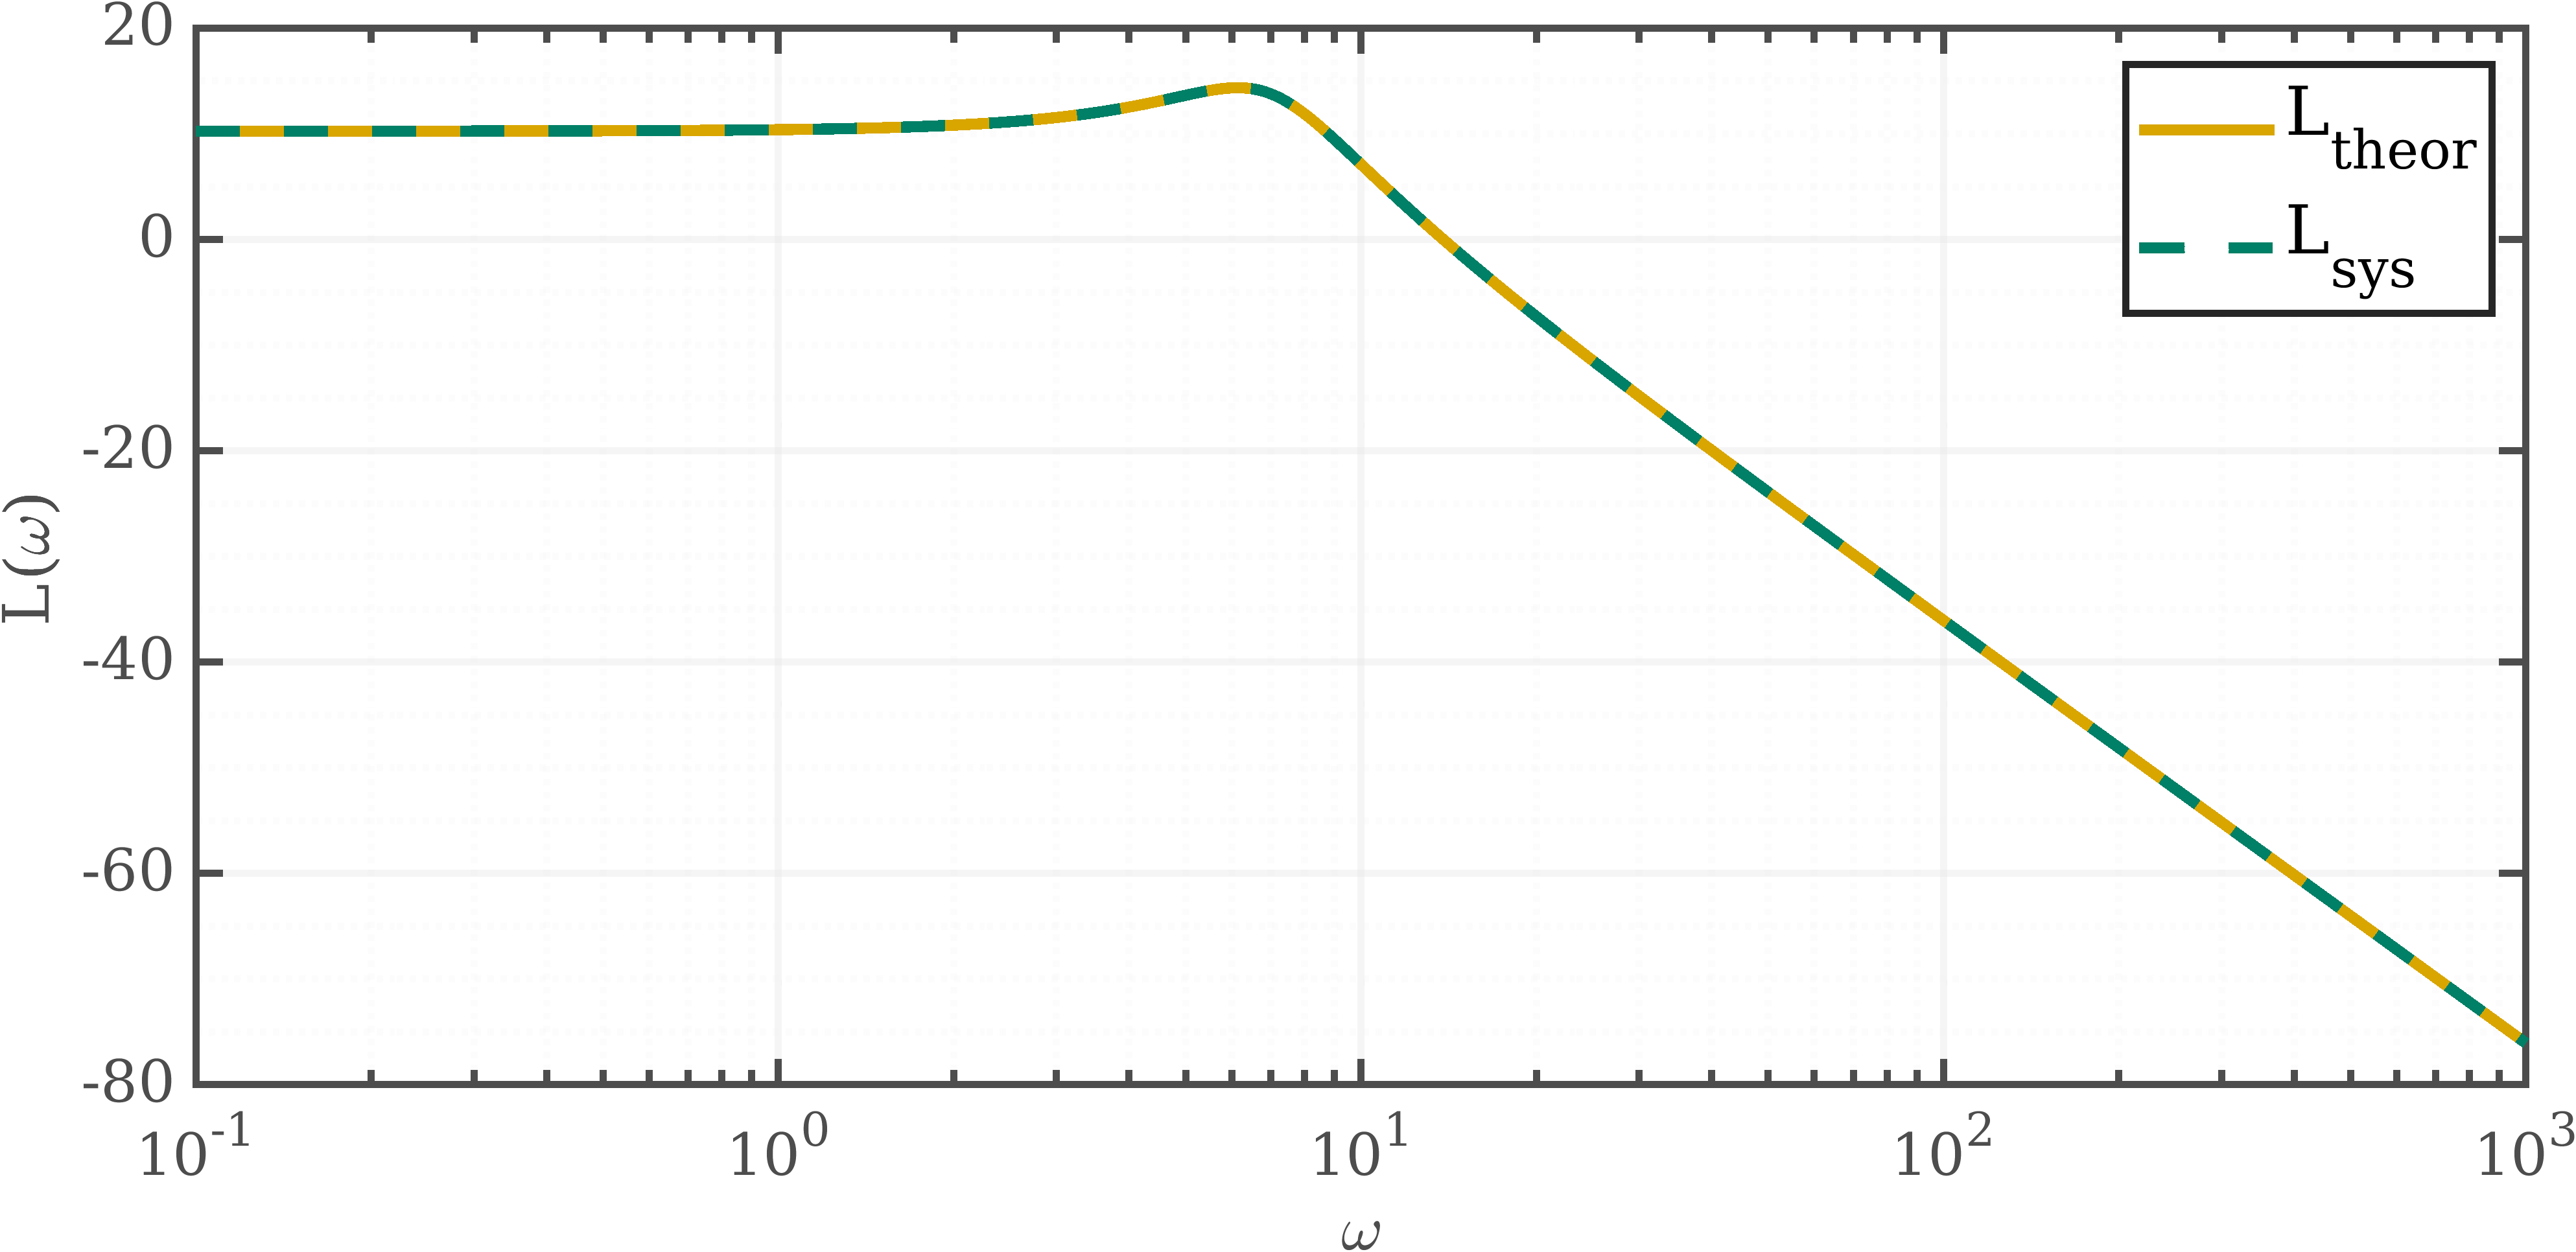
\includegraphics[width=0.9\textwidth]{../images/task2/freq/lach2.png}
		\caption{ЛАЧХ}
	\end{figure}	
	
	Также запишу ФЧХ для колебательного звена:
	
	\[
	\varphi(\omega)
	=
	-a\pi
	-
	\arctan\!\left(
	\frac{2\xi T\,\omega}{1 - \omega^{2} T^{2}}
	\right)
	\qquad
	a=
	\begin{cases}
		0, & \omega < T^{-1}\\[4pt]
		1, & \omega > T^{-1}
	\end{cases}
	\]
	
	\[
	\varphi(\omega)
	=
	-a\pi
	-
	\arctan\!\left(
	\frac{0.095\,\omega}{1 - 0.0207\,\omega^{2}}
	\right)
	\qquad
	a=
	\begin{cases}
		0, & \omega < 6.94\\[4pt]
		1, & \omega > 6.94
	\end{cases}
	\]
	
    \begin{figure}[H]
		\centering
		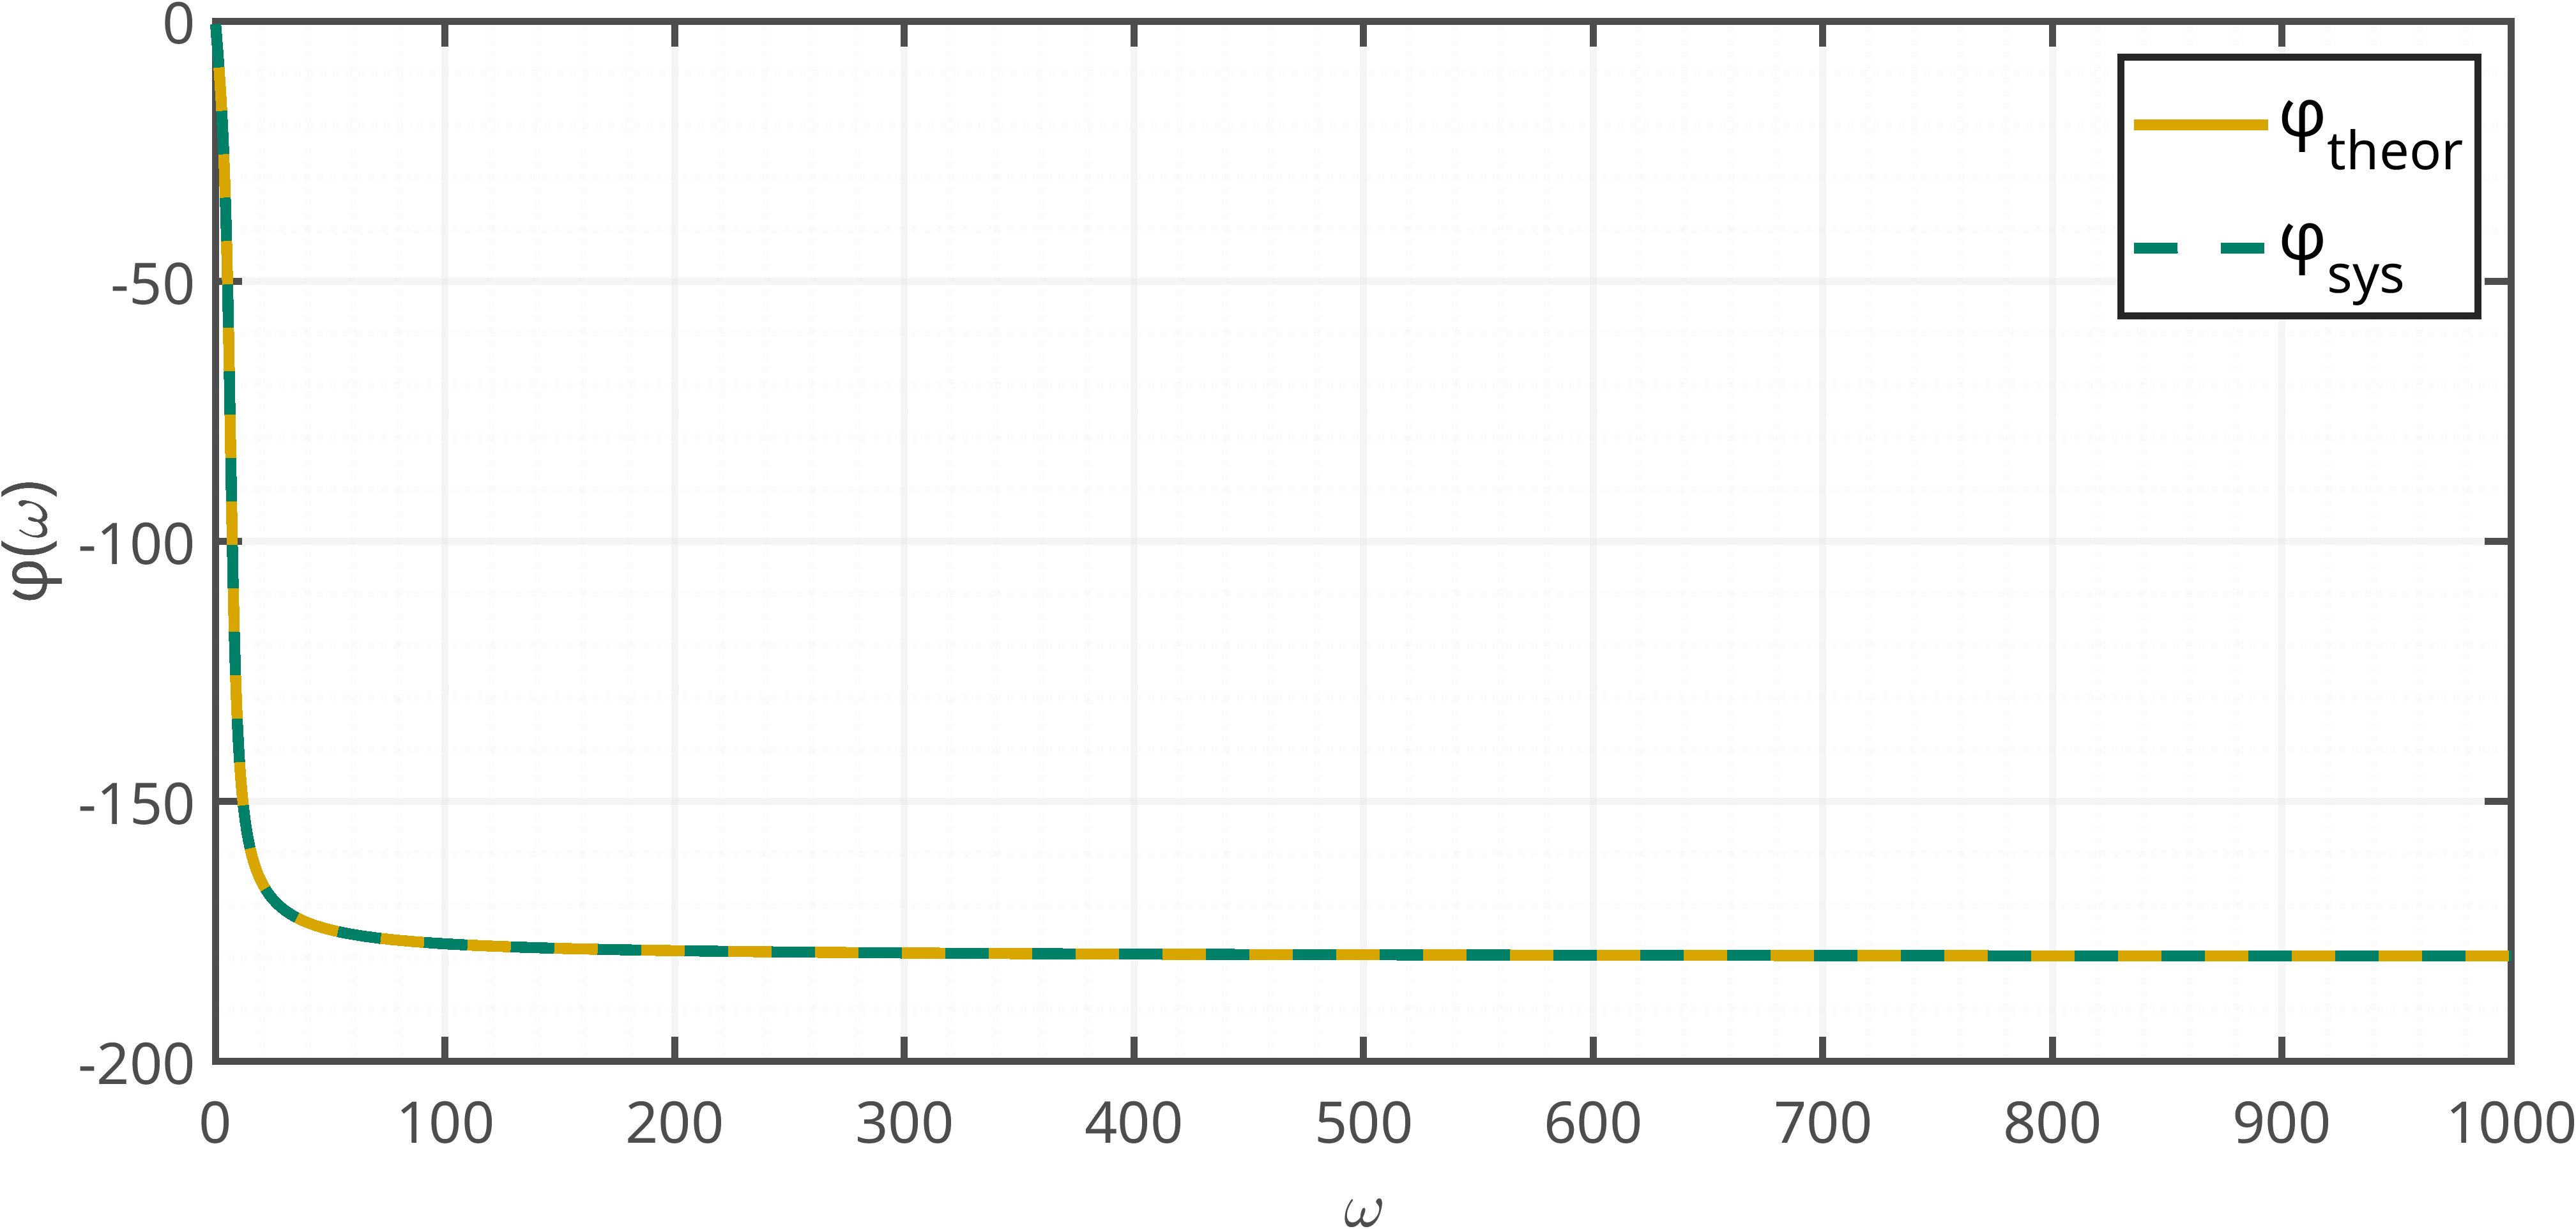
\includegraphics[width=0.9\textwidth]{../images/task2/freq/fch2.png}
		\caption{ФЧХ}
	\end{figure}	
	
	ЛФЧХ колебательного звена:
	
	\[
	\varphi(\omega)
	=
	-a\pi
	-
	\arctan\!\left(
	\frac{2\xi T\,\omega}{1 - \omega^{2} T^{2}}
	\right)
	\qquad
	a=
	\begin{cases}
		0, & \omega < T^{-1}\\[4pt]
		1, & \omega > T^{-1}
	\end{cases} 
	\quad \text{В координатах: }  \left( \log_{10}\omega,\; \varphi(\omega) \right)
	\]
	
	\[
	\varphi(\omega)
	=
	-a\pi
	-
	\arctan\!\left(
	\frac{0.095\,\omega}{1 - 0.0207\,\omega^{2}}
	\right)
	\qquad
	a=
	\begin{cases}
		0, & \omega < 6.94\\[4pt]
		1, & \omega > 6.94
	\end{cases}
	\quad \text{В координатах: }  \left( \log_{10}\omega,\; \varphi(\omega) \right)
	\]
	
	 \begin{figure}[H]
		\centering
		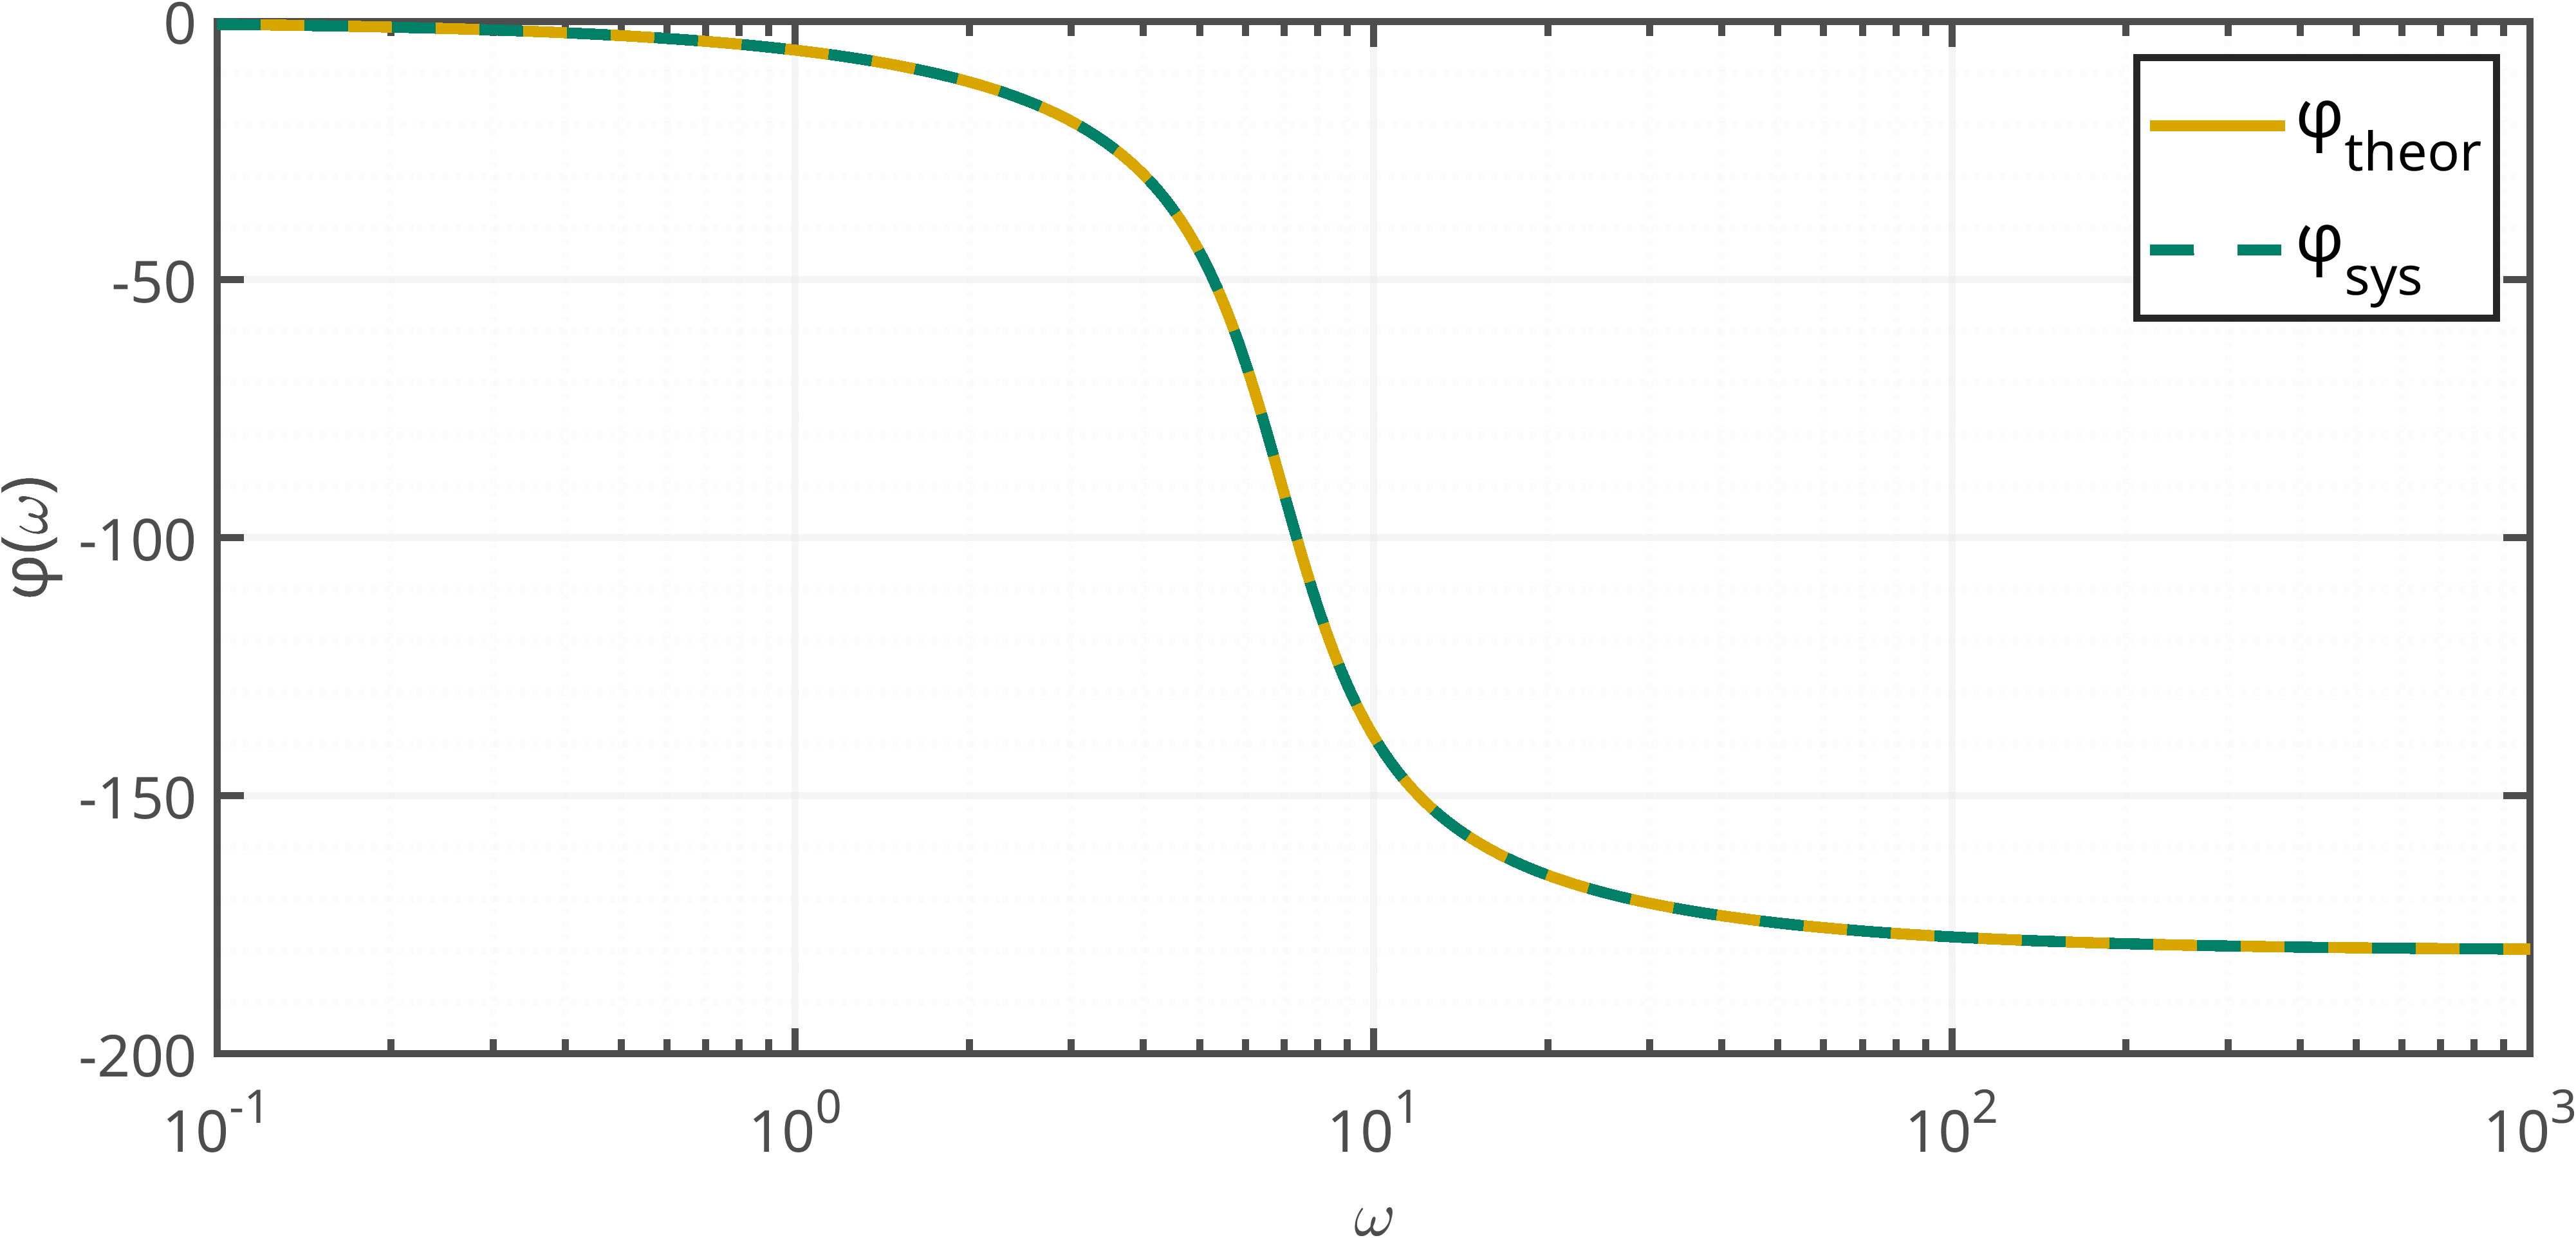
\includegraphics[width=0.9\textwidth]{../images/task2/freq/lfch2.png}
		\caption{ЛФЧХ}
	\end{figure}
	
	\textbf{Итог: }
	
	
	\newpage
	\section{Конденсатор}
	
	Запишу уравнение конденсатора: 
	\[
	I = C \frac{dU}{dt}
	\]
	
	Передаточная функция:
	
	\[
	W(s) = \frac{1}{Cs}
	\]
	
	При значении ёмкости \(C = 419\) передаточная функция имеет вид:
	\[
	W(s) = \frac{1}{419\,s}
	\]
	
	соответствует идеально интегрирующему звену с коэффициентом
	\[
	K = \frac{1}{419}
	\]
	
	\subsection{Временные характеристики}
	
	Для идеального интегрирующего звена известна весовая функция:
	
	\[w(t) = K = \frac{1}{419}\]
	
	\begin{figure}[H]
		\centering
		
\includegraphics[width=0.9\textwidth]{../images/task3/time/w3.png}
		\caption{Весовая функция}
	\end{figure}
	
	И переходная функция: 
	\[
	h(t)=K \cdot t = \frac{t}{419}\]
	
	\begin{figure}[H]
		\centering
		
\includegraphics[width=0.9\textwidth]{../images/task3/time/y3.png}
		\caption{Переходная функция}
	\end{figure}
	
	\subsection{Частотные характеристики}
	
	АЧХ будет равна:
	
	\[A(\omega) = \frac{K}{\omega} = \frac{1}{419\,\omega}\]
	
	\begin{figure}[H]
		\centering
		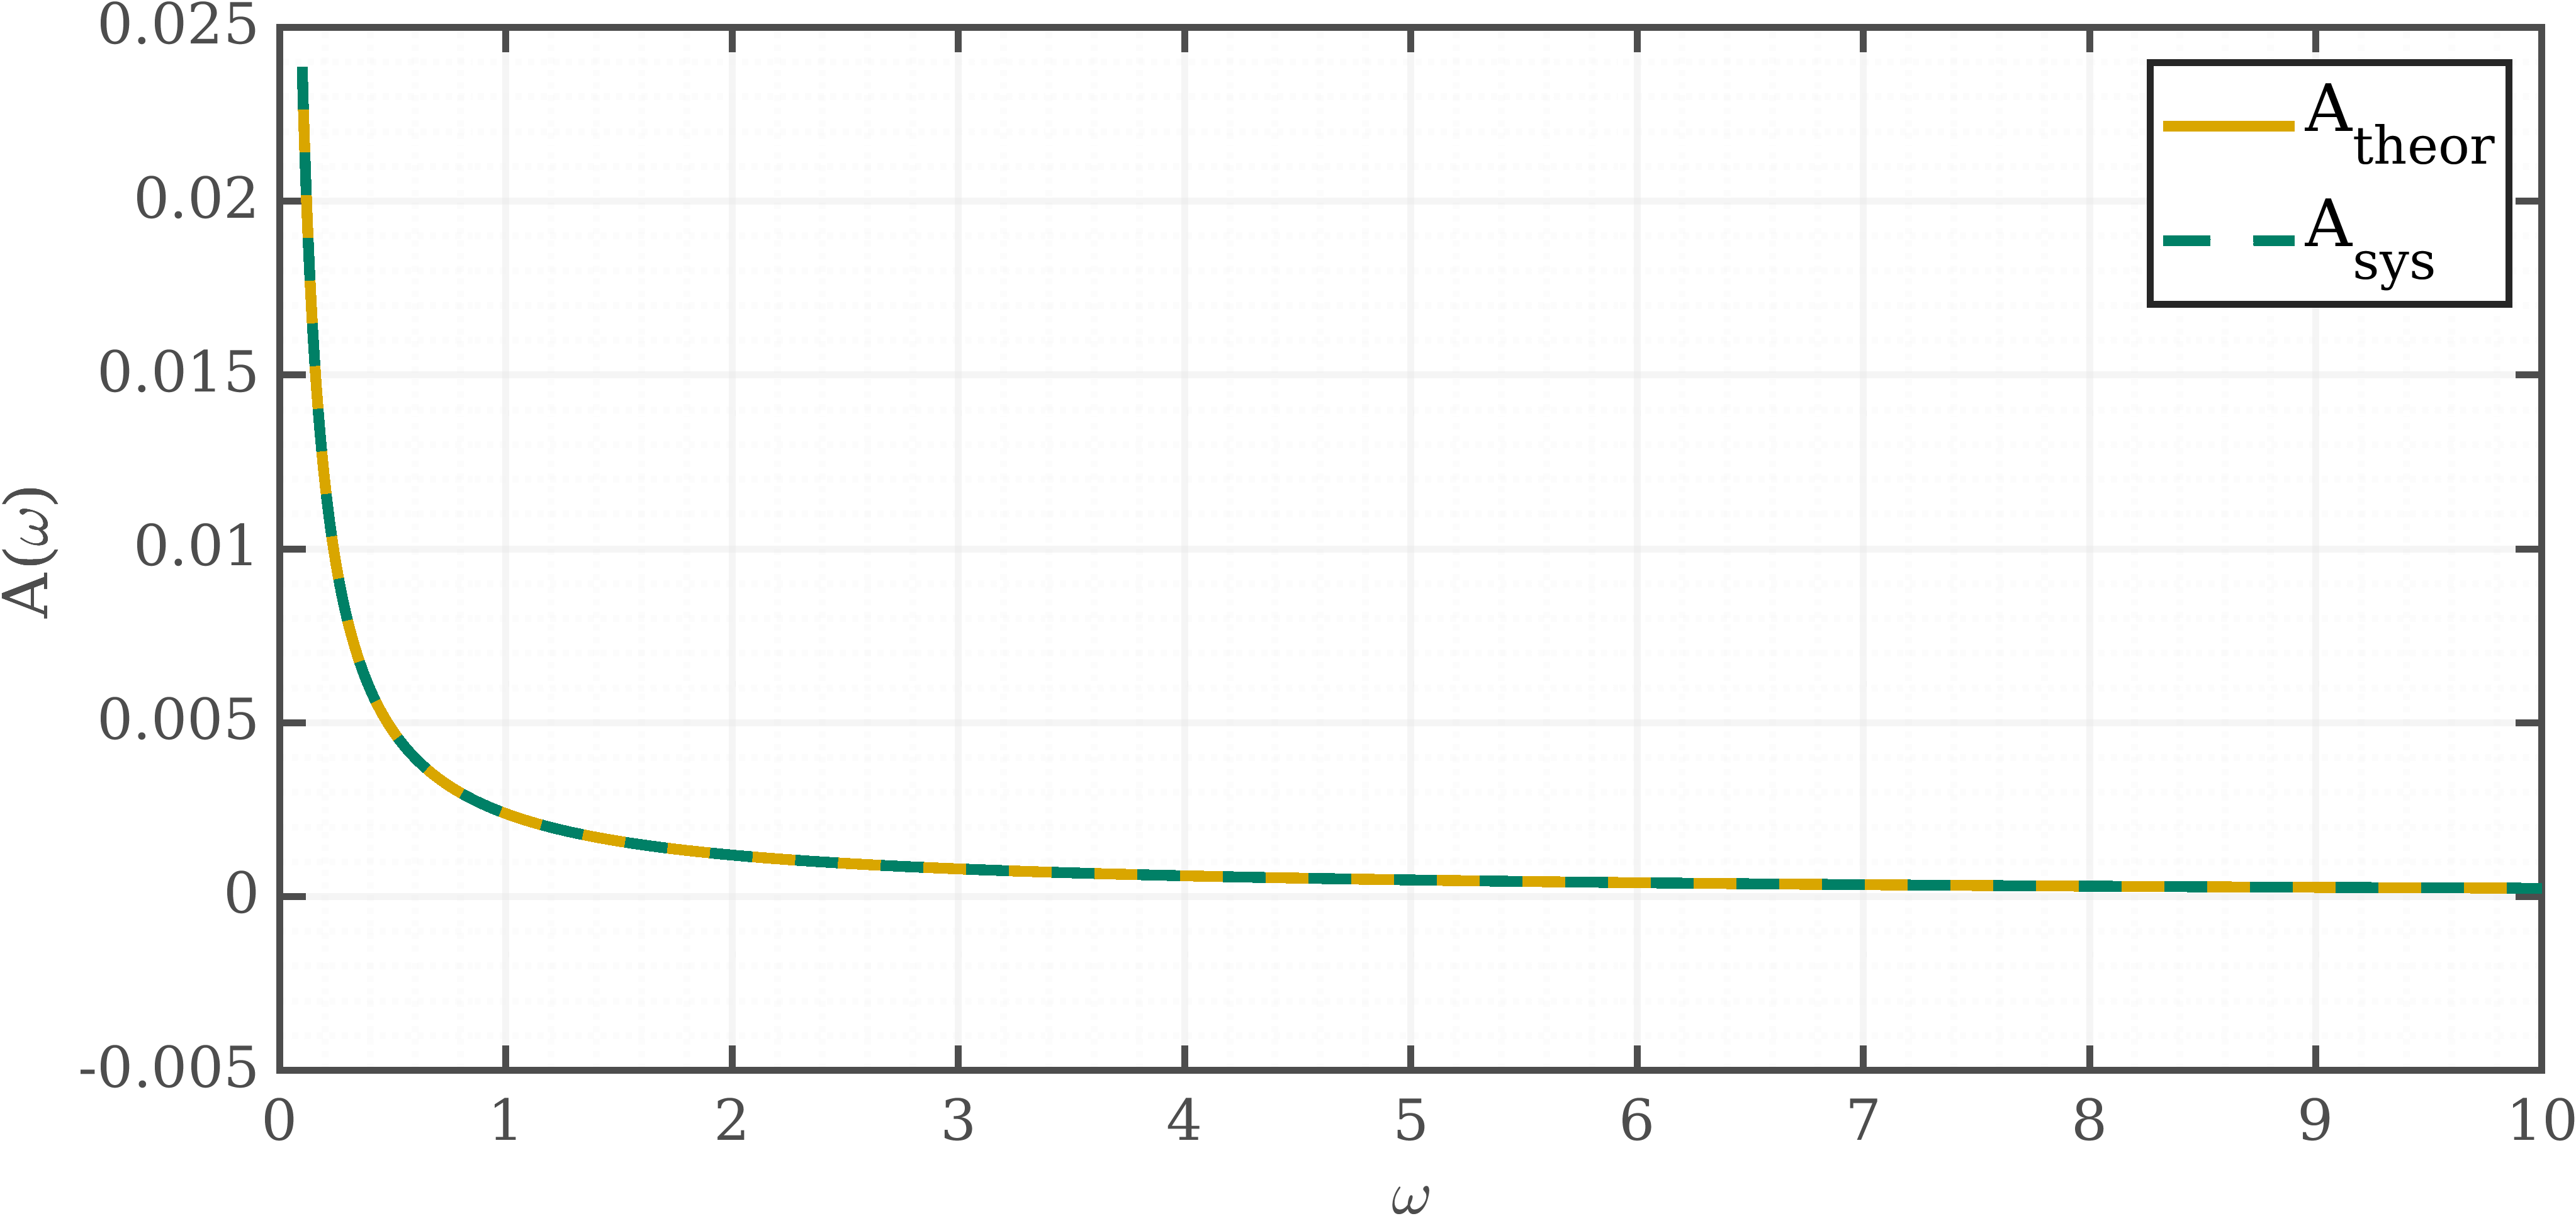
\includegraphics[width=0.9\textwidth]{../images/task3/freq/ach3.png}
		\caption{АЧХ}
	\end{figure}
	
	ЛАЧХ идеального интегрирующего звена:
	
	\[L(\omega) = 20\,lg(K) - 20\,lg(\omega) = 20\,lg(\frac{1}{419}) - 20\,lg(\omega)\]
	
	\begin{figure}[H]
		\centering
		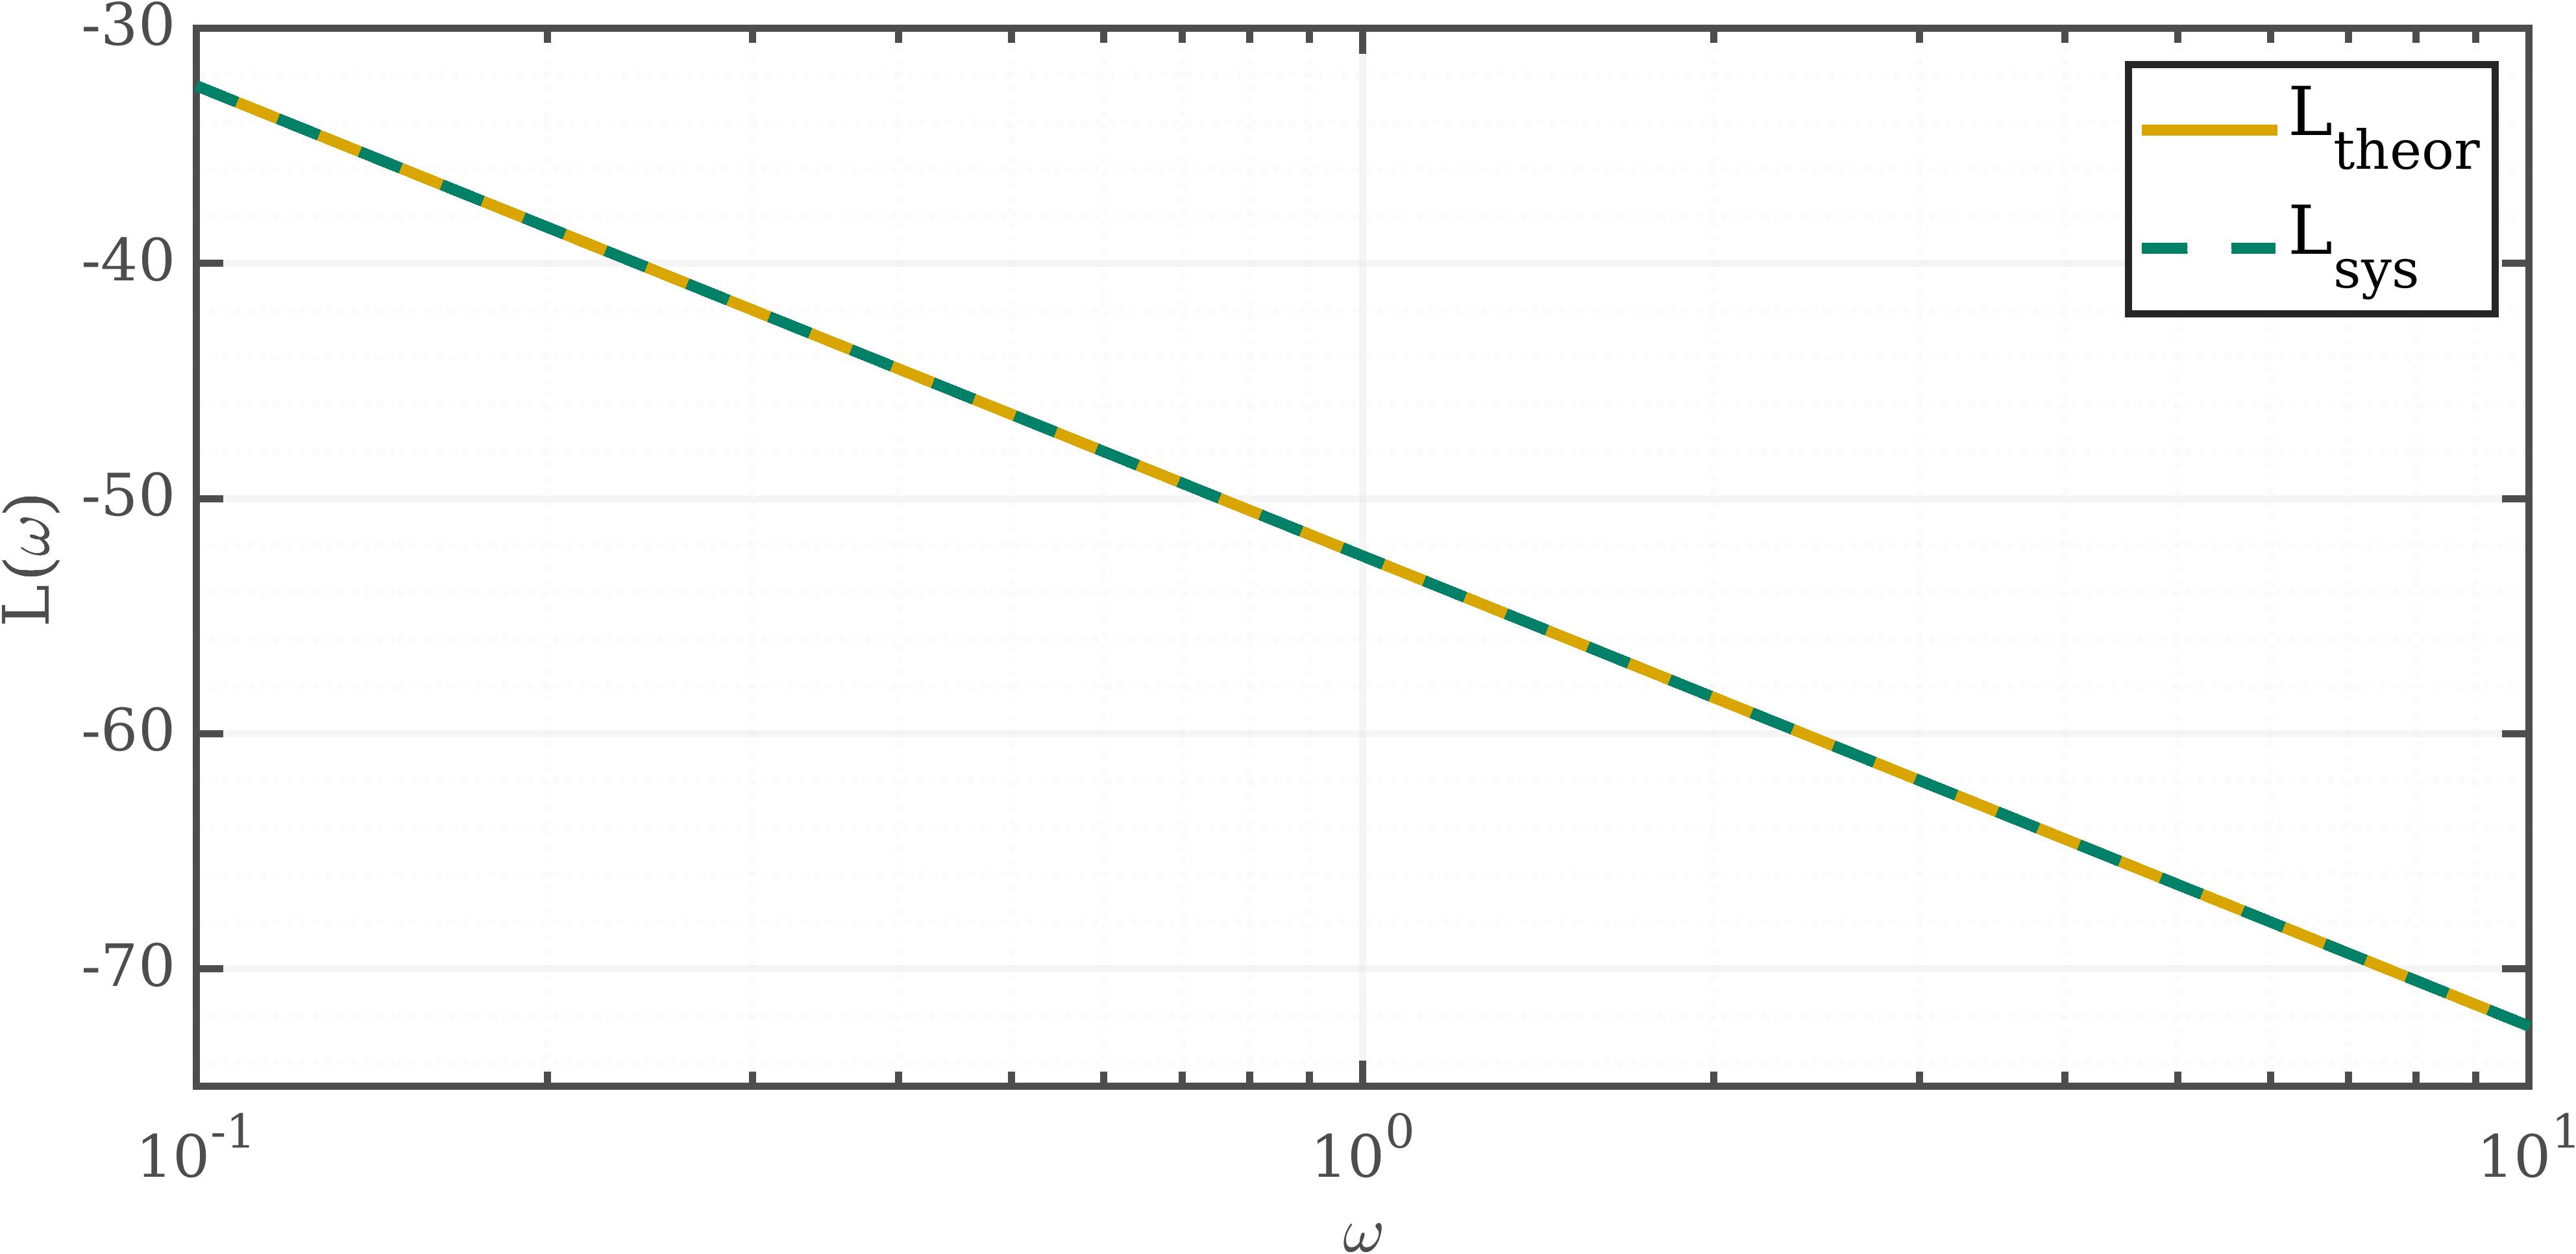
\includegraphics[width=0.9\textwidth]{../images/task3/freq/lach3.png}
		\caption{ЛАЧХ}
	\end{figure}
	
	Рассчитаю ФЧХ:
	
	\[\varphi(\omega) = \arctg(-\infty) = -\frac{\pi}{2}\]
	
	\begin{figure}[H]
		\centering
		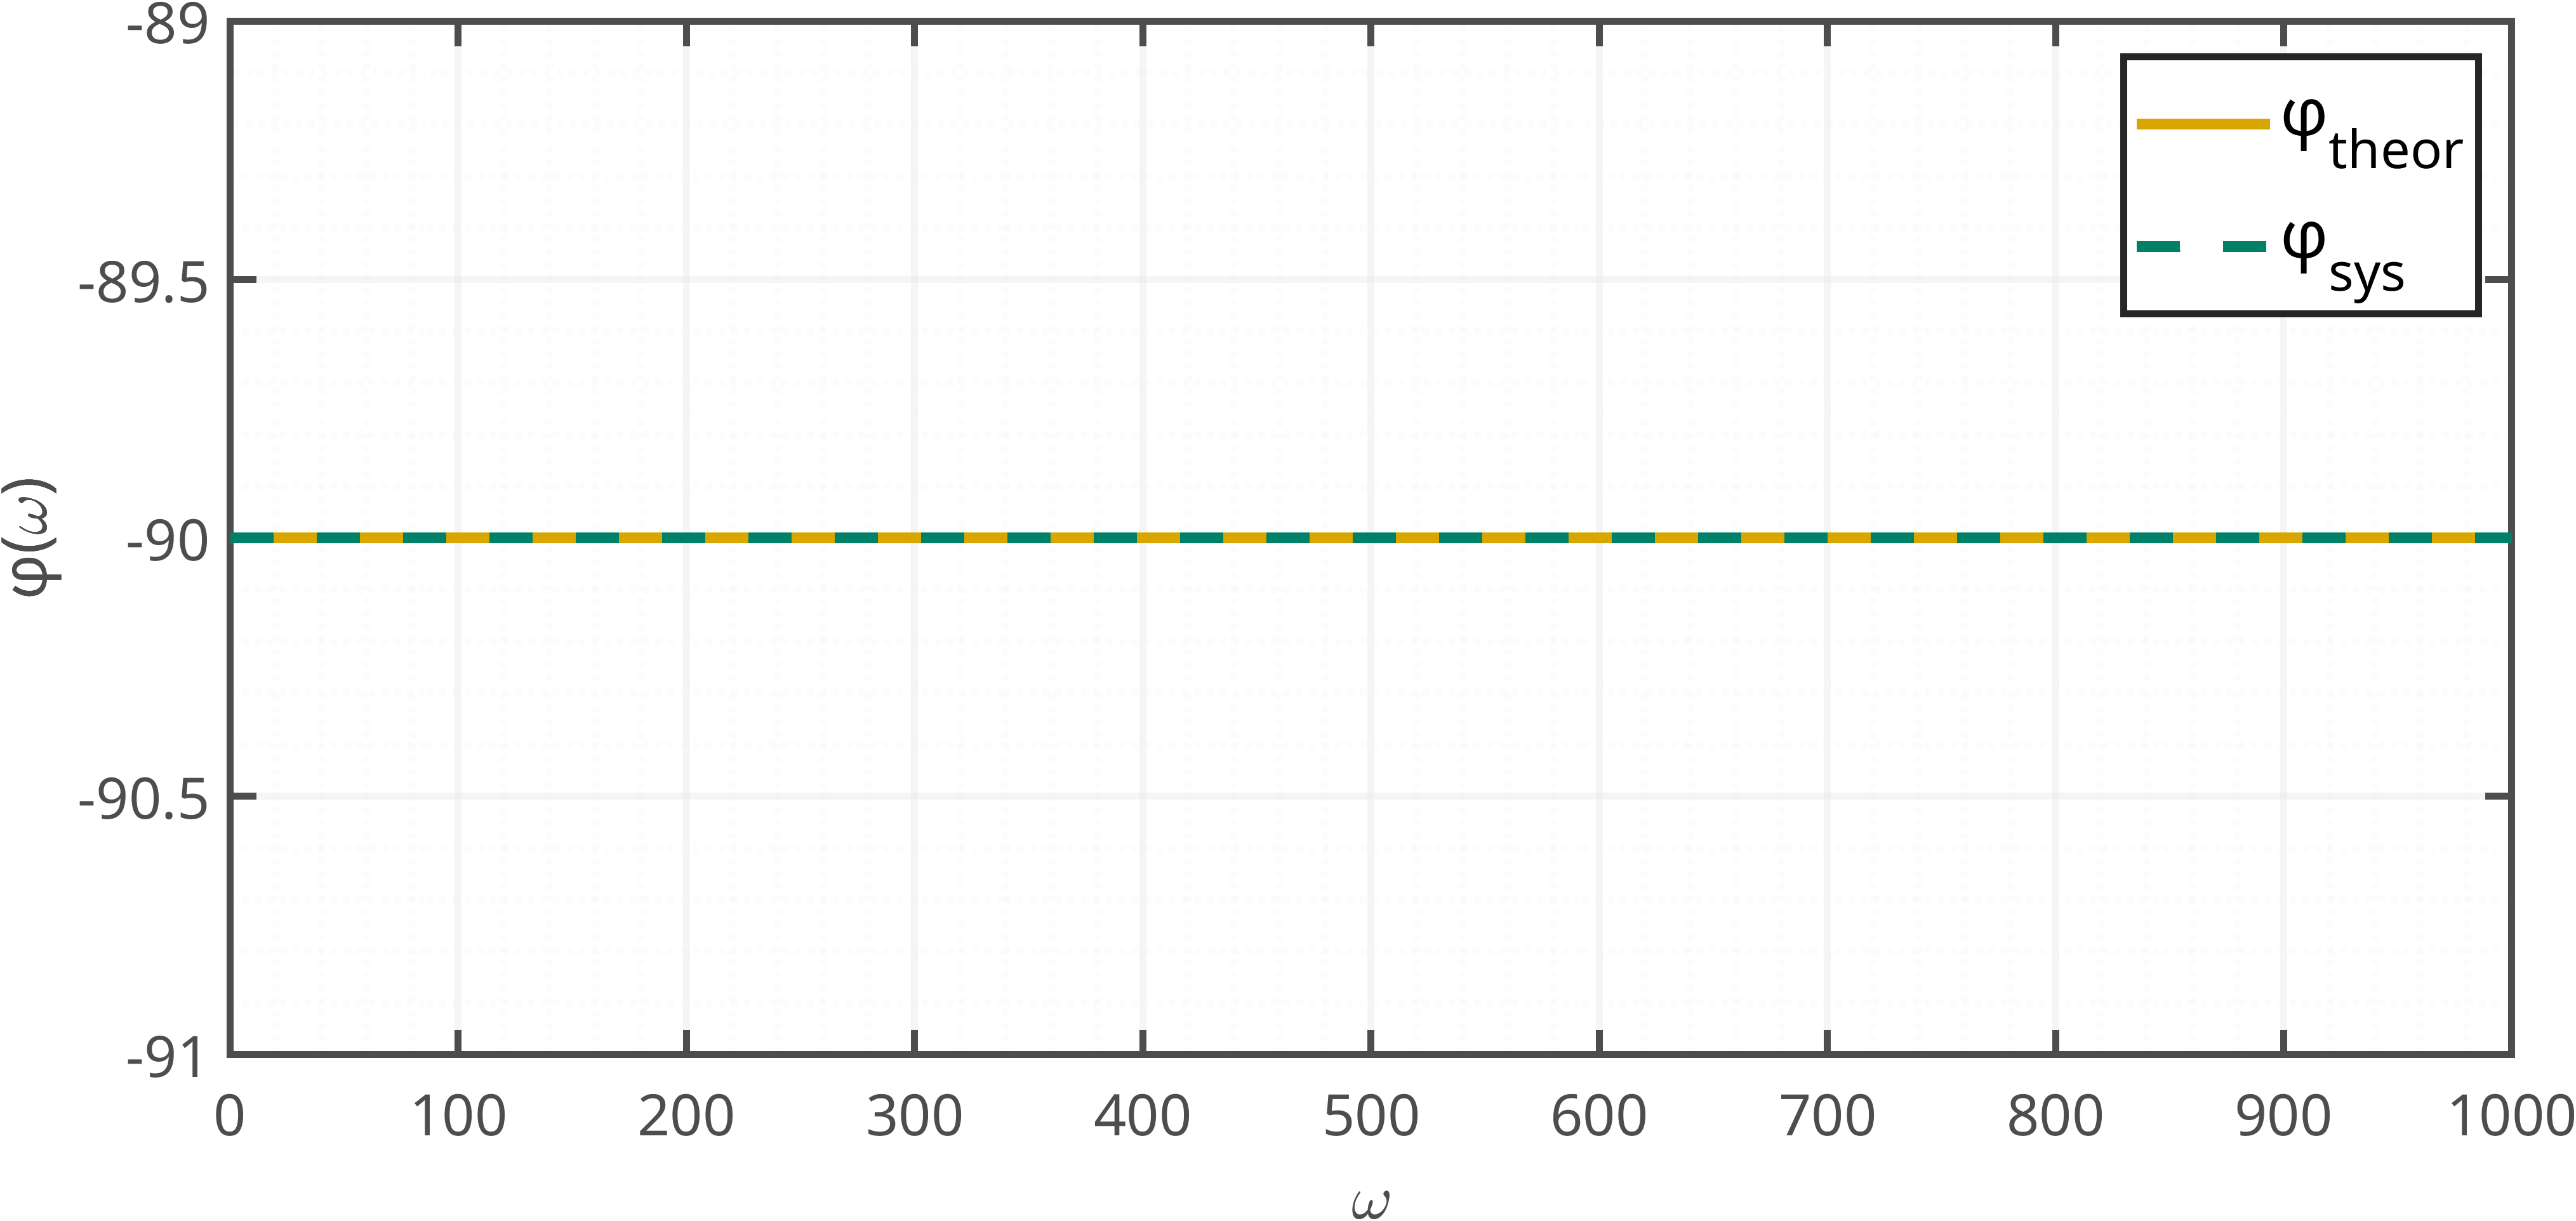
\includegraphics[width=0.9\textwidth]{../images/task3/freq/fch3.png}
		\caption{ФЧХ}ФЧХ
	\end{figure}
	
	ЛФЧХ идеального интегрирующего звена совпадает с обычной фазо-частотной характеристикой,
	поскольку фаза не зависит от частоты. Поэтому
	
	\[
	\varphi_{\lg}(\omega)
	=
	\varphi(\omega)
	=
	-\,\frac{\pi}{2}
	\]
	
	\begin{figure}[H]
		\centering
		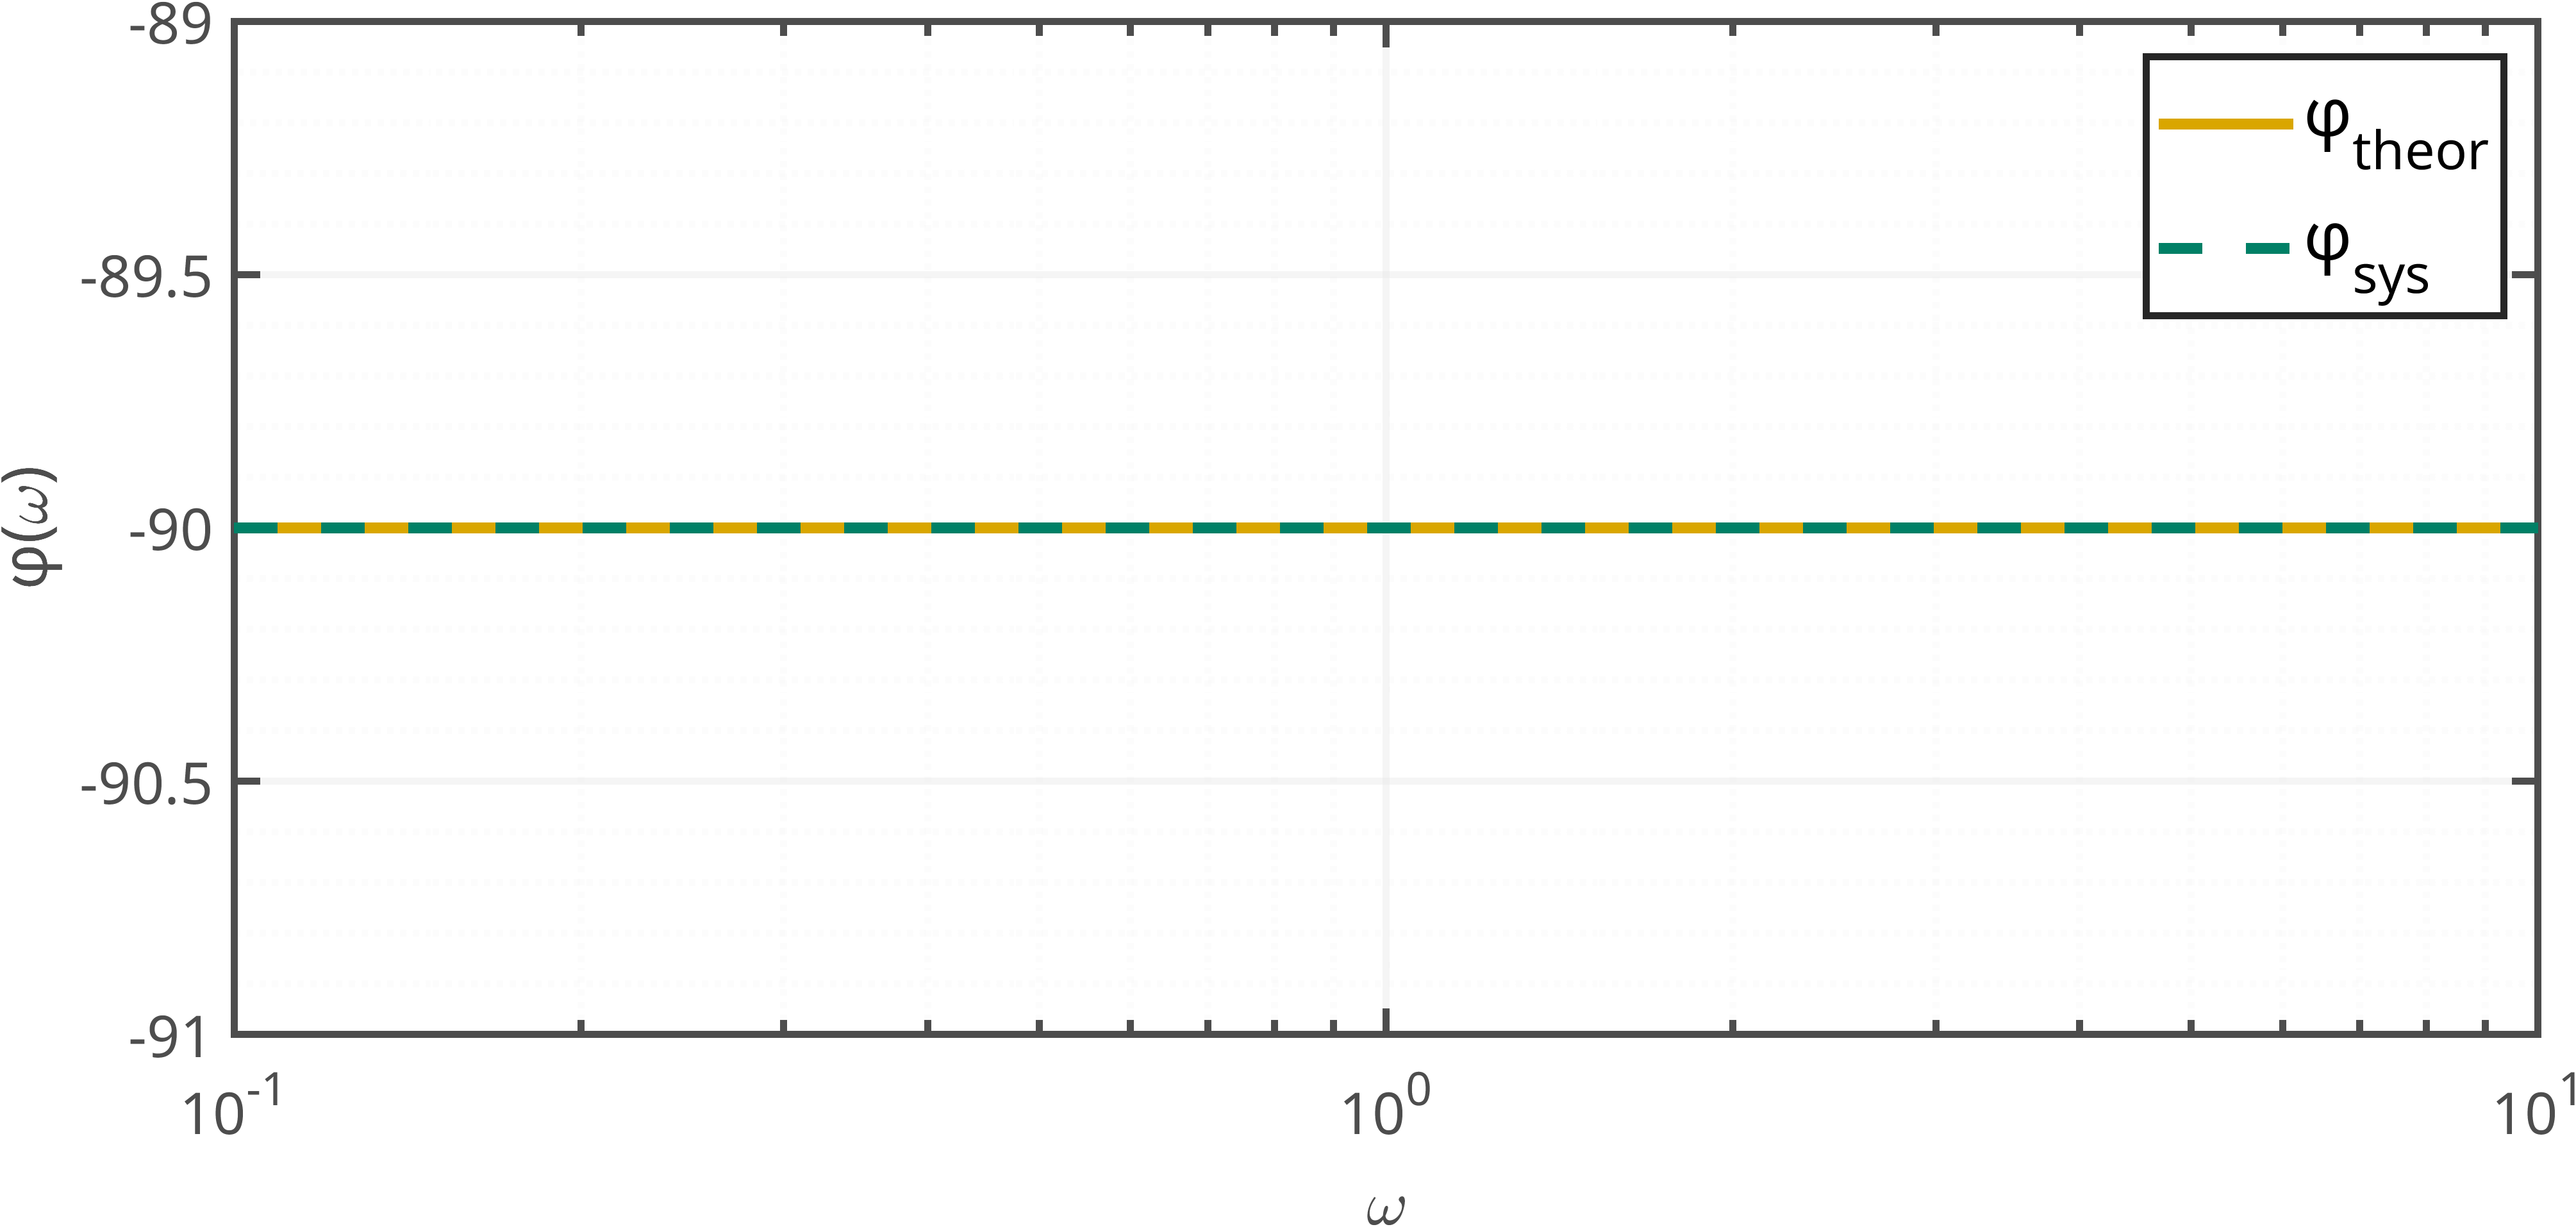
\includegraphics[width=0.9\textwidth]{../images/task3/freq/lfch3.png}
		\caption{ЛФЧХ}
	\end{figure}
	
	\textbf{Итог: } 
	
	
	\newpage
	\section{Пружина}
	
	\begin{figure}[h!]
		\centering
		\begin{tikzpicture}[scale=1.2, line width=1pt]
			
			\draw (0,0) -- (0,2);
			\foreach \y in {0.1,0.3,...,1.9}{
				\draw (-0.2,\y) -- (0,\y+0.2);
			}
			
			\draw (0,0) -- (5,0);
			
			\draw[decorate, decoration={coil, aspect=0.5, segment length=5pt, amplitude=4pt}]
			(0,1) -- (2,1);
			
			\node[orange] at (1,1.3) {$k$};
			
			\draw[fill=blue!40] (2,0.3) rectangle (3.5,1.7);
			\node[white] at (2.75,1.0) {\Large $M$};
			
			\foreach \x in {0.1,0.3,...,5}{
				\draw (\x,0) -- (\x+0.15,-0.25);
			}
			
			\draw[->,red, line width=1.4pt] (3.5,1) -- (4.7,1);
			\node[red] at (4.8,1.2) {$F$};
			
		\end{tikzpicture}
		\caption{Пружинный маятник}
	\end{figure}
	
	
	Запишу уравнения для пружинного маятника:
	
	\[F_\text{упр} = -k \cdot x \quad F = m \cdot a\]
	
	Дифференциальное уравнение пружинного маятника:
	\[
	m\ddot{x} + kx = u(t)
	\]
	
	Передаточная функция:
	\[
	W(s) = \frac{1}{ms^2 + k} = \frac{1/k}{m/k \cdot s^2 + 1}
	\]
	
	Согласно моему варианту:
	
	\[
	W(s) = \frac{1}{14s^2 + 71}
	\]
	
	Тип звена передаточной функции -- консервативное. Параметры:
	
	\[K = \frac{1}{k} = \frac{1}{71} \qquad T = \sqrt{\frac{m}{k}} = \sqrt{\frac{14}{71}}\]
	
	\subsection{Временные характеристики}
	
	Весовая функция консервативного звена известна и равна:
	
	\[w(t) = \frac{K}{T}\,sin(\frac{t}{T}) = \frac{1}{\sqrt{71 \cdot 14}}\,\sin\!\left(\sqrt{\frac{71}{14}}\,t\right)\]
	
	\begin{figure}[H]
		\centering
		
\includegraphics[width=0.9\textwidth]{../images/task4/time/w4.png}
		\caption{Весовая функция}
	\end{figure}
	
	Переходная функция для консервативного звена равна:
	\[
	h(t) = K\left(1 - \cos\!\left(\frac{t}{T}\right)\right)
	= \frac{1}{k}\left(1 - \cos\!\left(\sqrt{\frac{k}{m}}\,t\right)\right) = \frac{1}{71}\left(1 - \cos\!\left(\sqrt{\frac{71}{14}}\,t\right)\right)
	\]

	\begin{figure}[H]
		\centering
		
\includegraphics[width=0.9\textwidth]{../images/task4/time/y4.png}
		\caption{Переходная функция}
	\end{figure}

	\subsection{Частотные характеристики}
	
	Запишу формулу для АЧХ консервативного звена:
	
	\[
	A(\omega) = \frac{K}{\left| 1 - \omega^{2} T^{2} \right|}
	= \frac{1}{71\,\left| 1 - \dfrac{14}{71}\,\omega^{2} \right| }
	\]
	
	\begin{figure}[H]
		\centering
		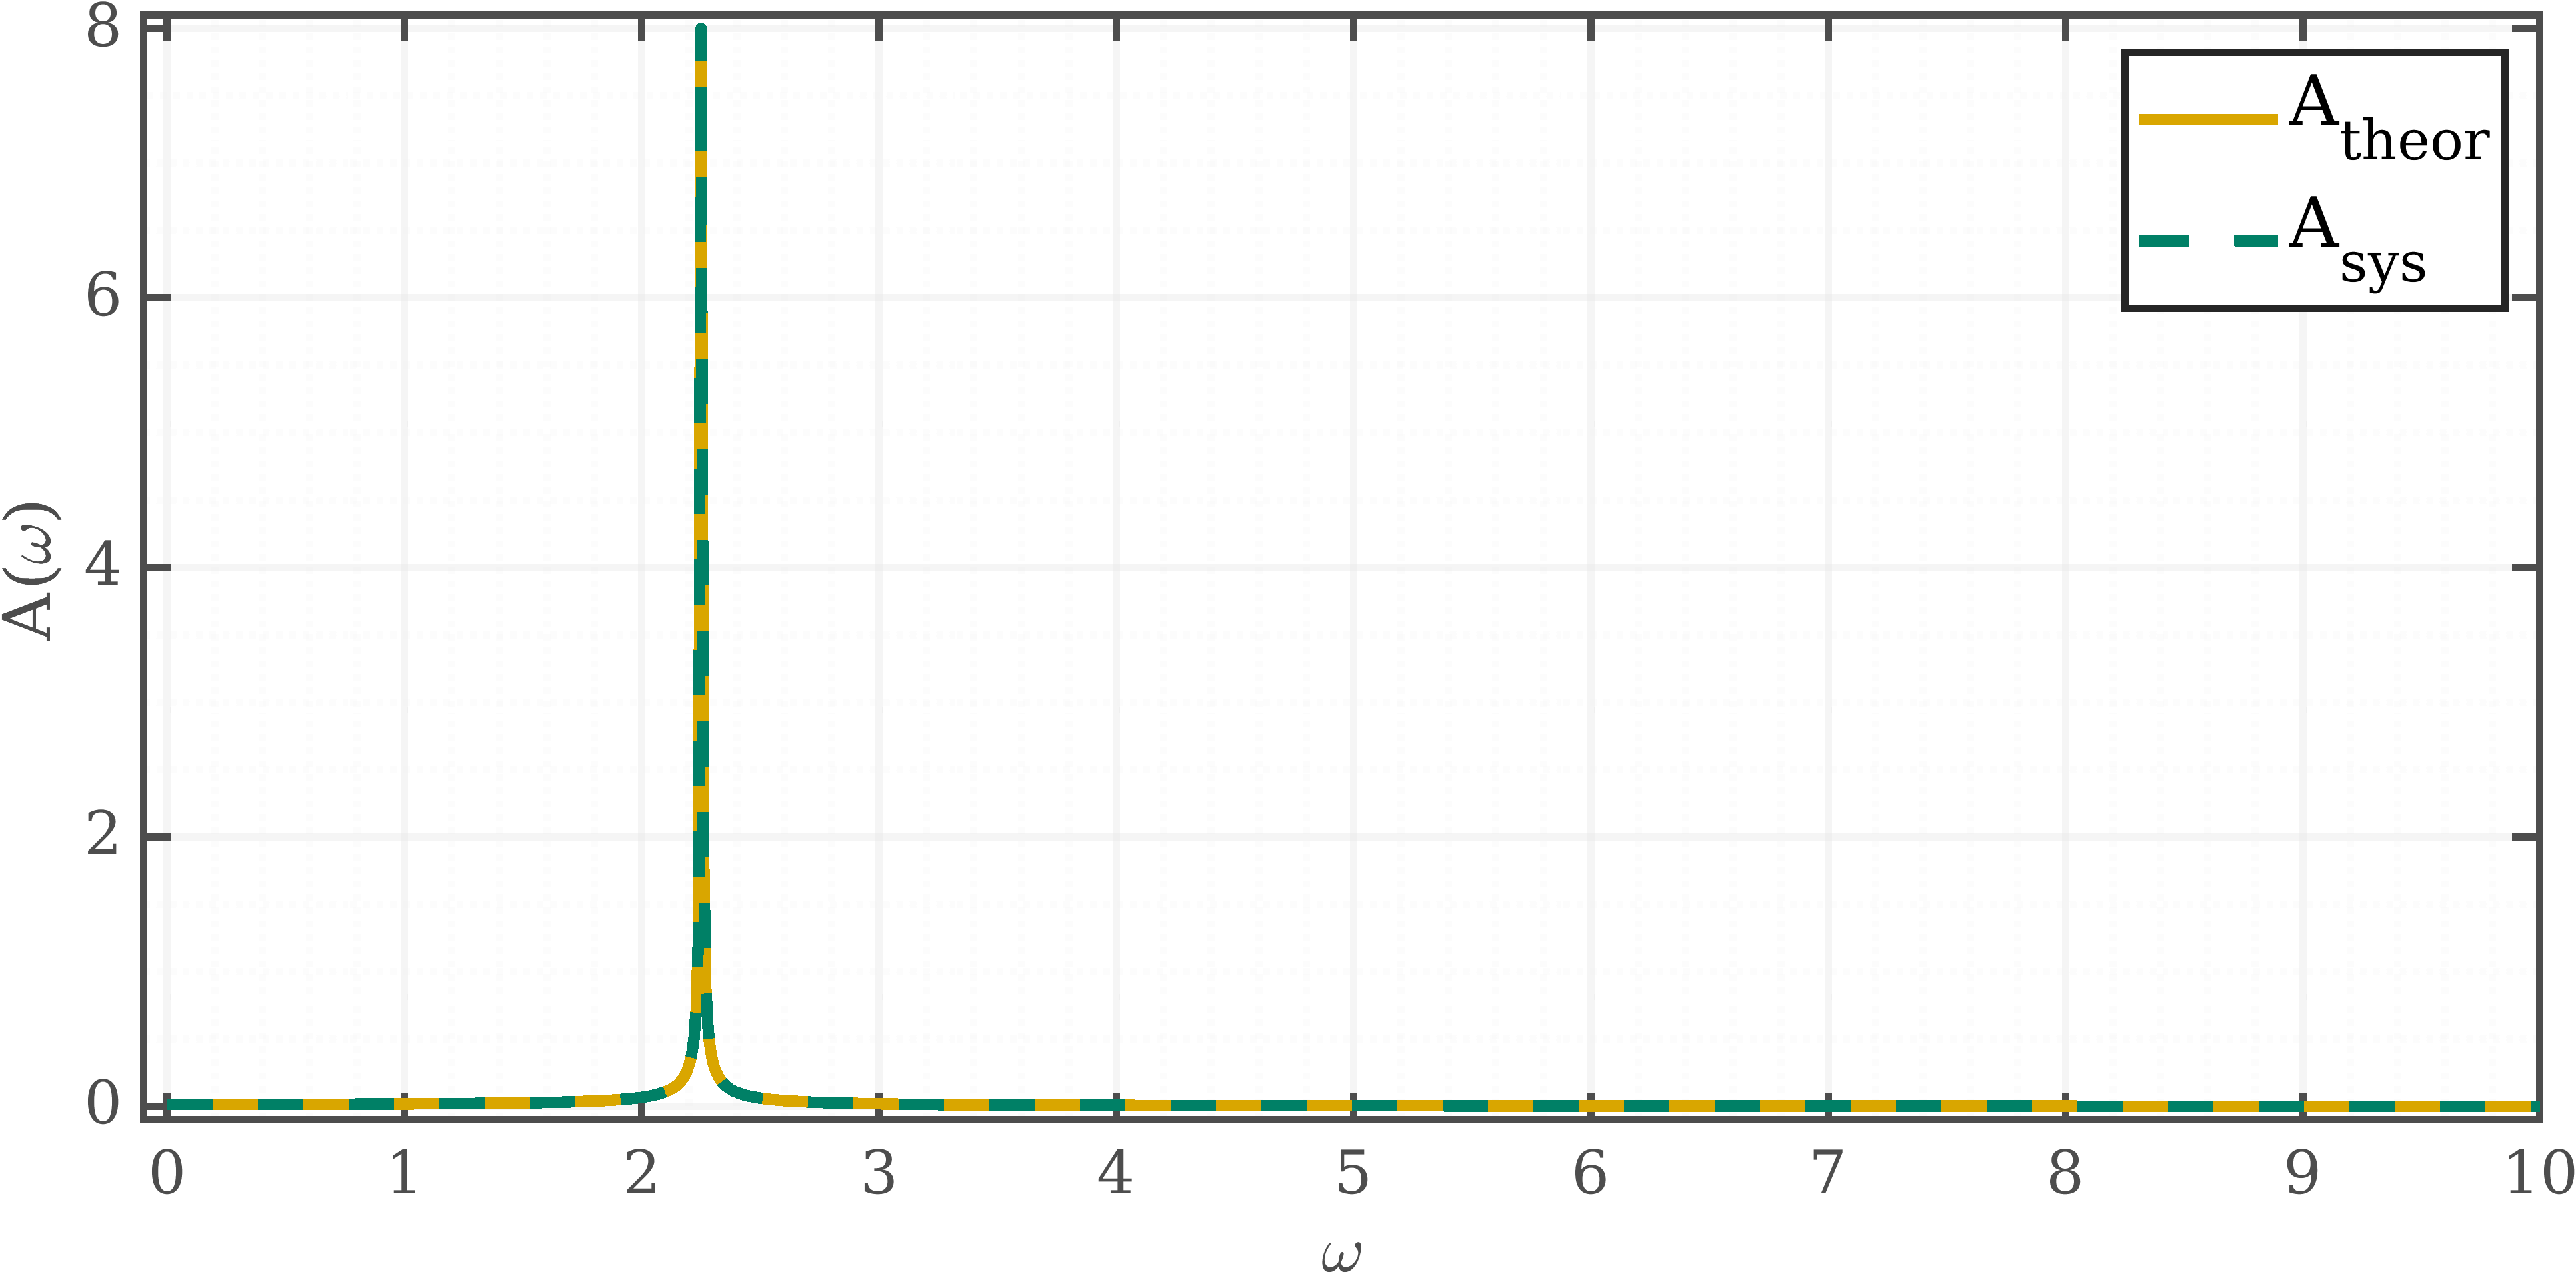
\includegraphics[width=0.9\textwidth]{../images/task4/freq/ach4.png}
		\caption{АЧХ}
	\end{figure}
	
	Логарифмическая амплитудно-частотная характеристика консервативного звена:
	
	\[
	L(\omega)
	= 20\lg K - 20\lg\!\left|1 - \omega^2 T^2\right| = 20\lg\left(\frac{1}{71}\right)
	- 20\lg\left|1 - \frac{14}{71}\,\omega^2\right|
	\]
	
	\begin{figure}[H]
		\centering
		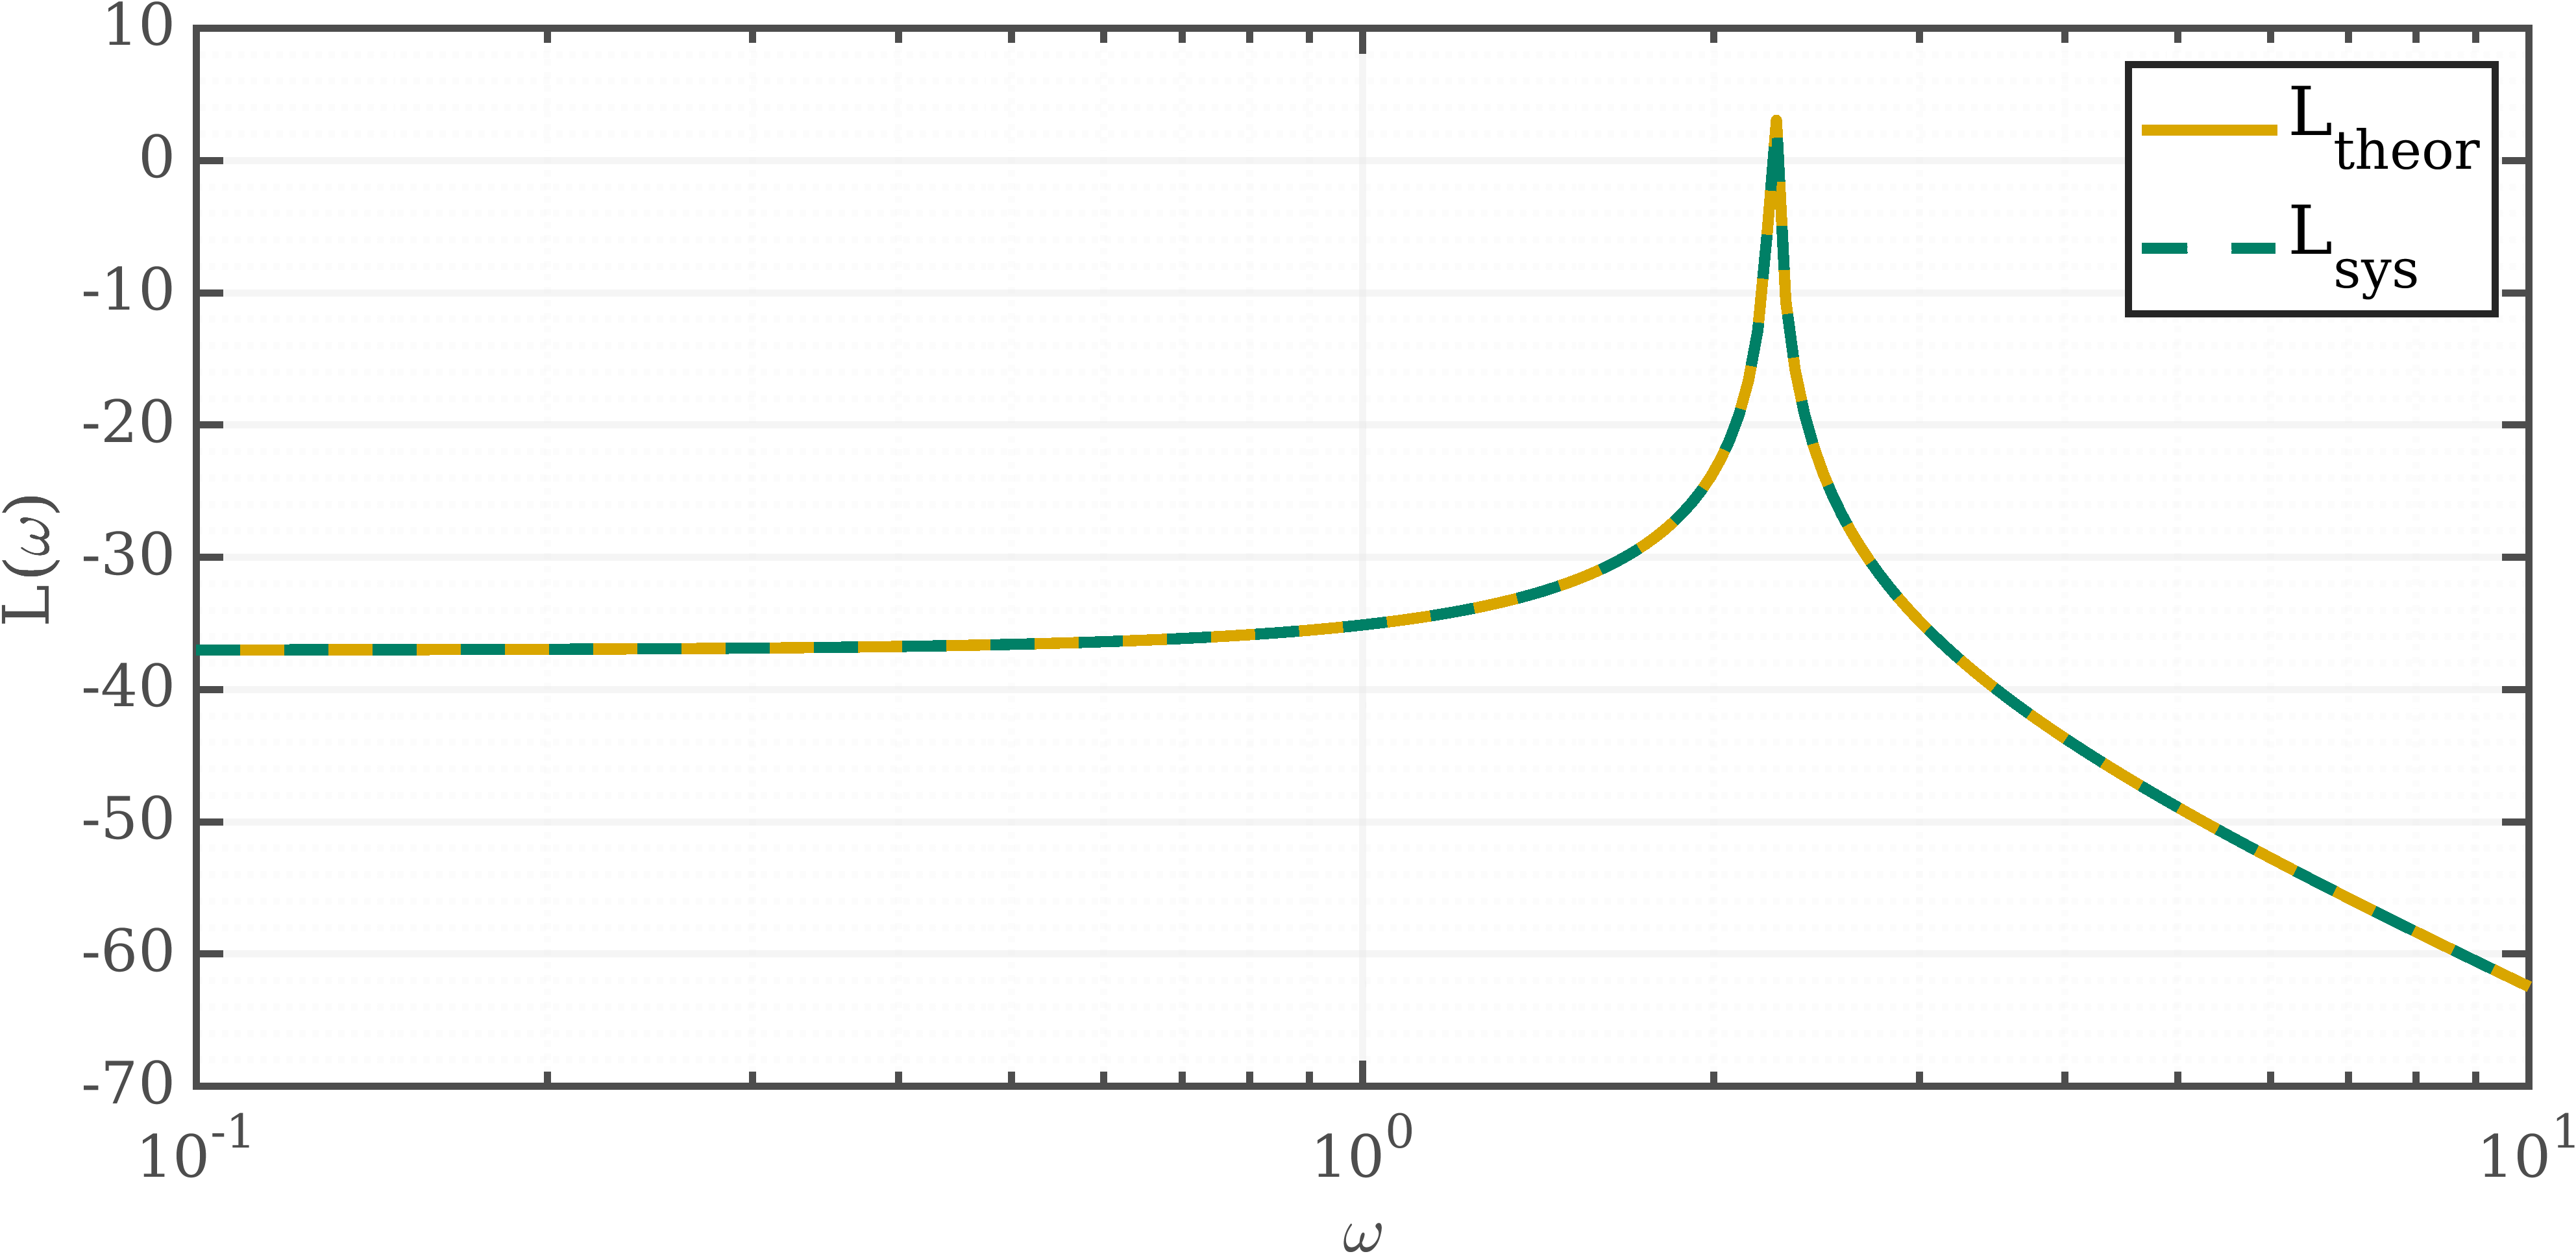
\includegraphics[width=0.9\textwidth]{../images/task4/freq/lach4.png}
		\caption{ЛАЧХ}
	\end{figure}
	
	ФЧХ дя консервативного звена:
	
	\[
	\varphi(\omega) = -a\pi \qquad
	\begin{cases}
		a = 0 & \omega < T^{-1} \\
		a = 1 & \omega > T^{-1}
	\end{cases} 
	\quad \Longrightarrow \quad
	\begin{cases}
		a = 0 & \omega < \sqrt{\dfrac{71}{14}} \\[8pt]
		a = 1 & \omega > \sqrt{\dfrac{71}{14}}
	\end{cases}
	\]
	
	\begin{figure}[H]
		\centering
		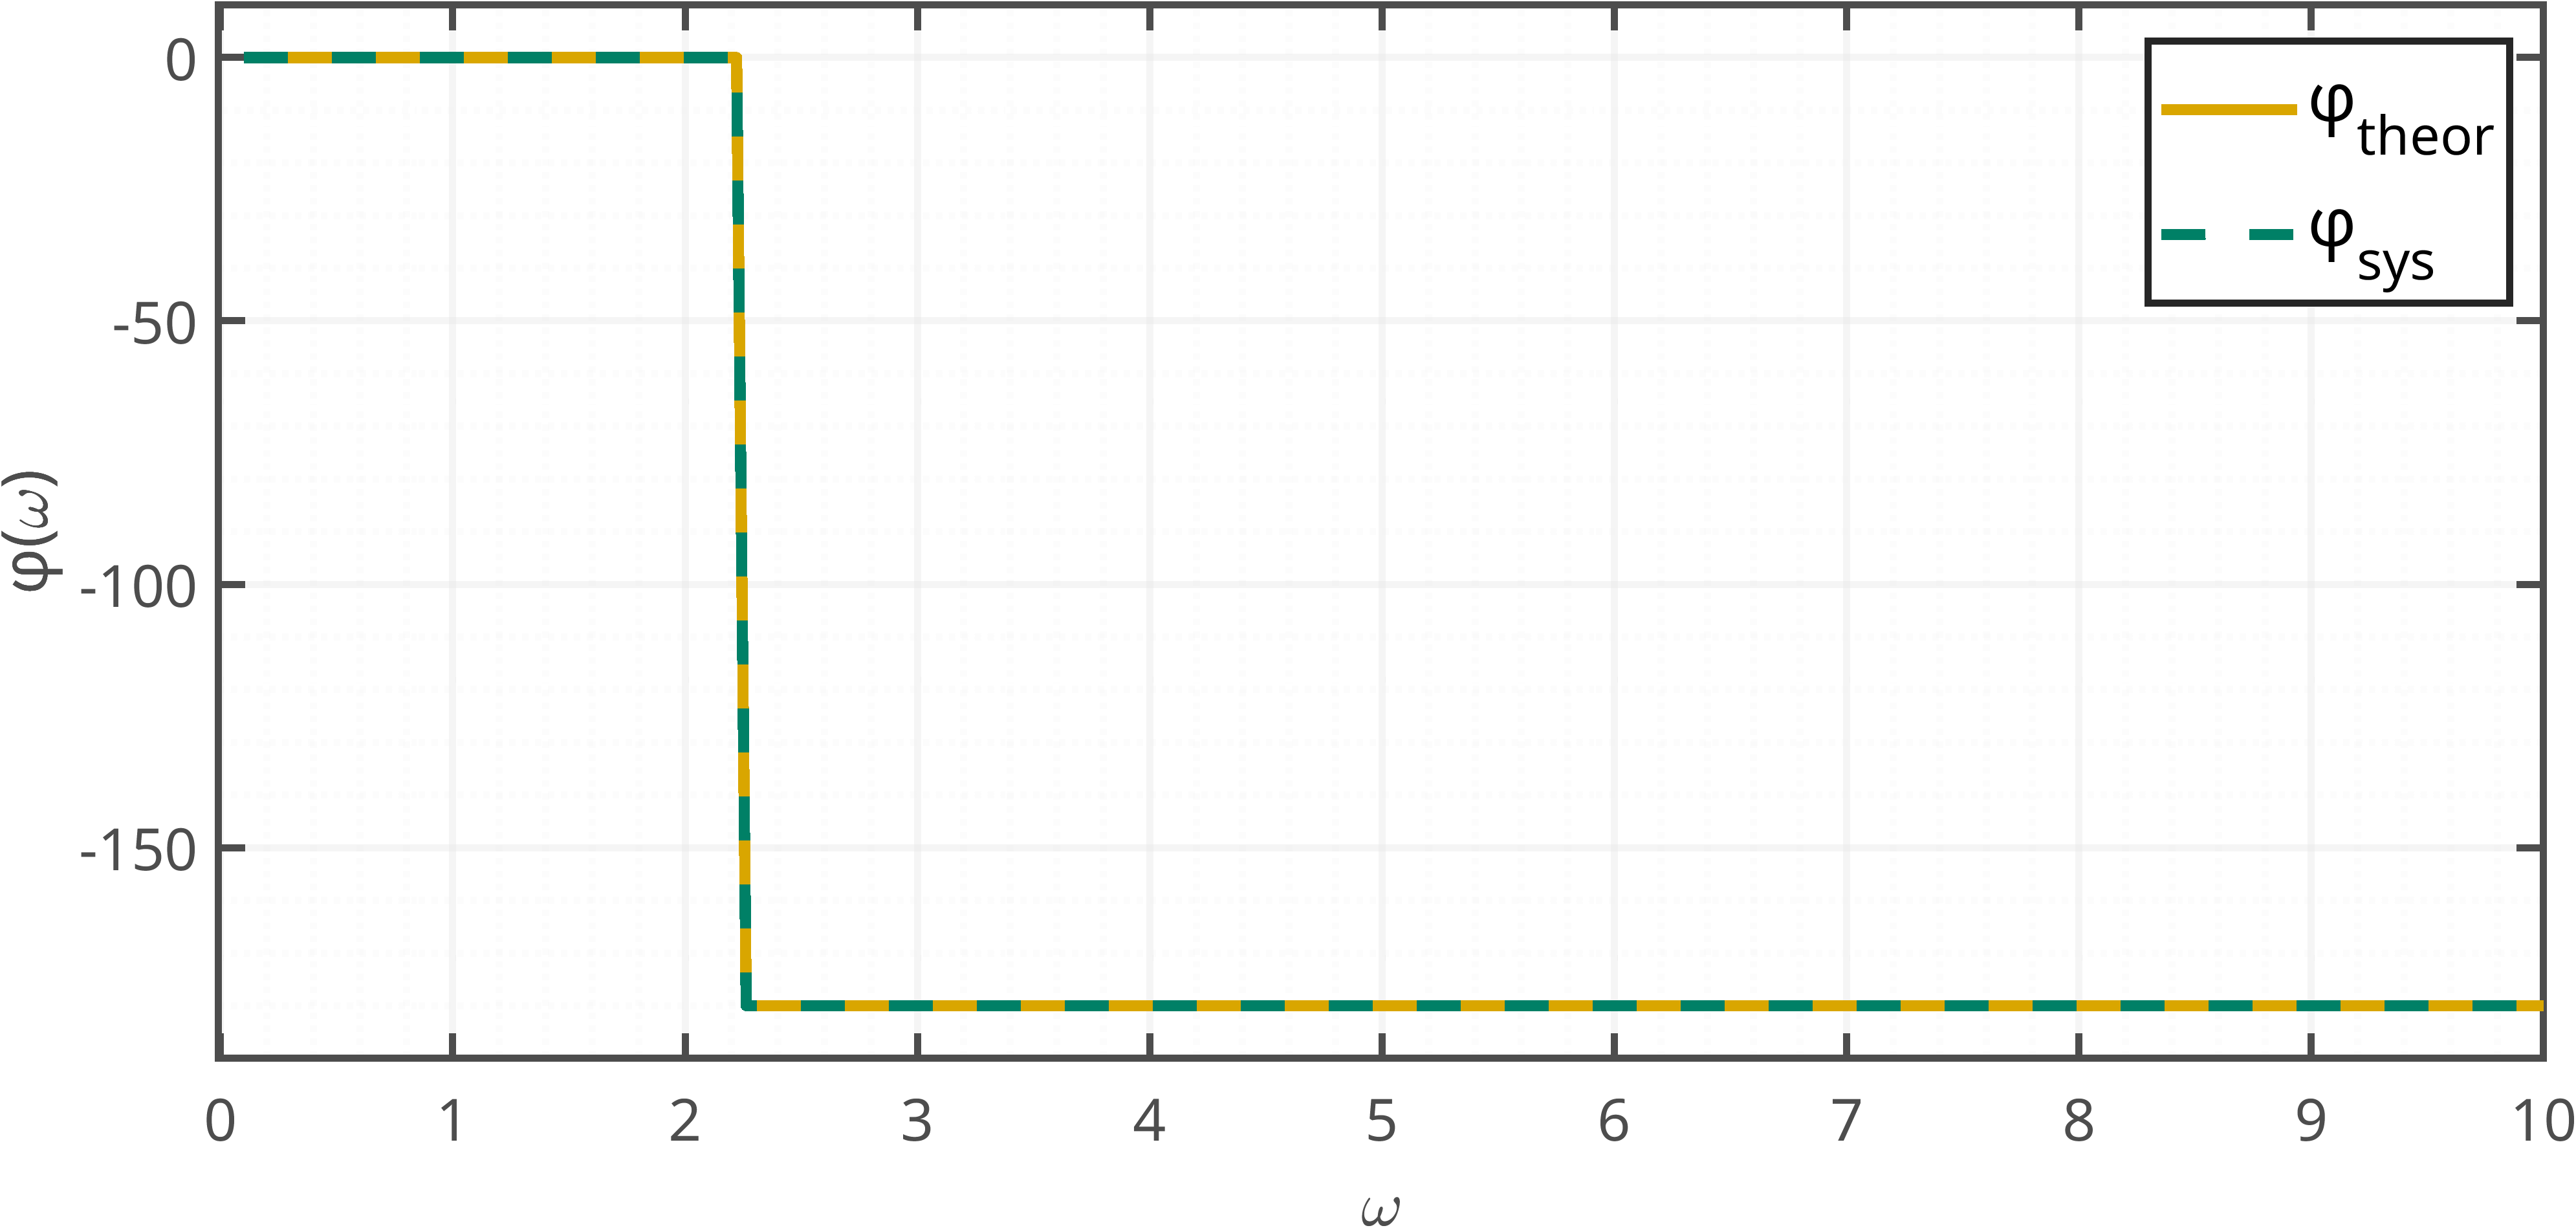
\includegraphics[width=0.9\textwidth]{../images/task4/freq/fch4.png}
		\caption{ФЧХ}
	\end{figure}
	
	Тогда ЛФЧХ имеет вид:
	\[
	\varphi(\omega) = -a\pi \qquad
	\begin{cases}
		a = 0 & \omega < \sqrt{\dfrac{71}{14}} \\[8pt]
		a = 1 & \omega > \sqrt{\dfrac{71}{14}}
	\end{cases} \quad \text{В координатах:} \quad \left( \log_{10}\omega,\; \varphi(\omega) \right)
	\]
	
	\begin{figure}[H]
		\centering
		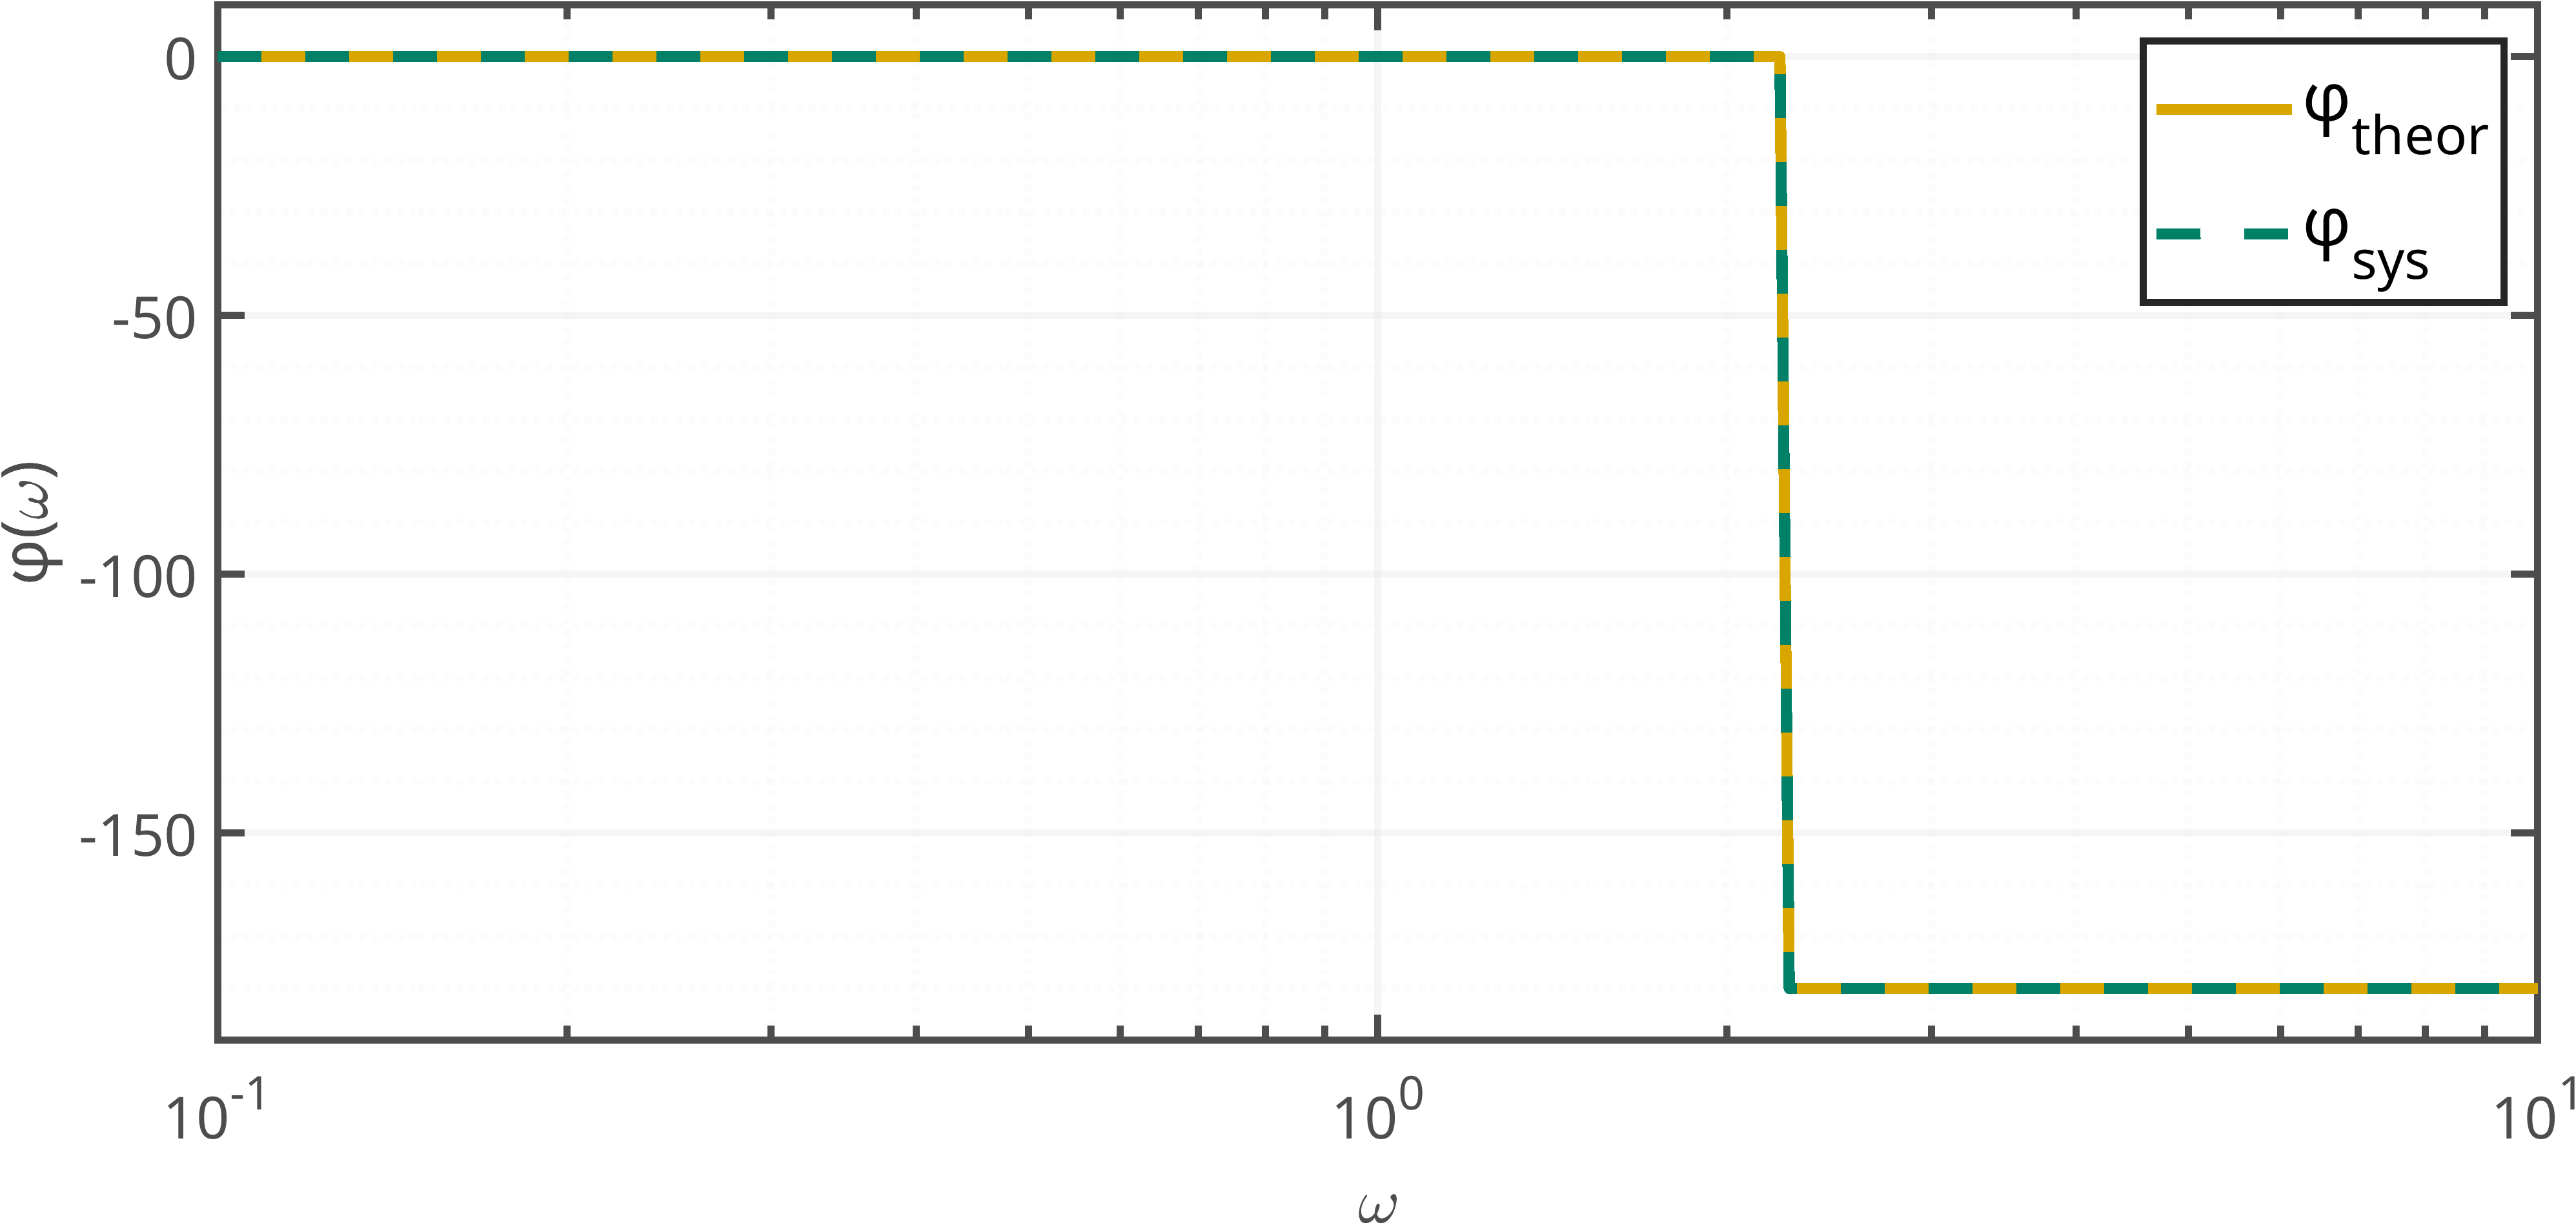
\includegraphics[width=0.9\textwidth]{../images/task4/freq/lfch4.png}
		\caption{ЛФЧХ}
	\end{figure}
	
	\textbf{Итог: }
	
	\newpage
	\section{Регулятор на операционном усилителе}
	
	
	
	\subsection{Временные характеристики}
	\subsection{Частотные характеристики}


	\newpage
	\section{Вывод}

	Материалы работы: \href{https://github.com/decadeos/ITMO/tree/master/3_course/lsau/lab5}{\texttt{github.com}}

\end{document}